\documentclass[11pt]{article}

\usepackage[a4paper,left=2.0cm,right=2.0cm,top=2.3cm,bottom=2.3cm]{geometry}
\usepackage{ctex}
\usepackage{amsmath,amssymb,bm}
\usepackage{graphicx}
\usepackage{float}
\usepackage{subcaption}
\usepackage{booktabs}
\usepackage{multirow}
\usepackage{siunitx}
\usepackage[inline]{enumitem}
\usepackage[colorlinks=true,linkcolor=blue,urlcolor=blue]{hyperref}

\setmainfont{Palatino Linotype}
\setCJKmainfont{SimSun}[BoldFont=SimHei,ItalicFont=KaiTi]
\setCJKsansfont{SimHei}
\sisetup{separate-uncertainty=true}
\graphicspath{{Figure/}{analysis_output/}}

\newcommand{\experiName}{布朗运动的统计特性与扩散系数测定}
\newcommand{\supervisor}{彭毅}
\newcommand{\name}{邓思豪}
\newcommand{\studentNum}{2023K8009909008}
\newcommand{\class}{3}
\newcommand{\group}{01}
\newcommand{\seat}{5}
\newcommand{\dateYear}{2026}
\newcommand{\dateMonth}{6}
\newcommand{\dateDay}{1、8}
\newcommand{\room}{西实验楼204}
\newcommand{\others}{$\square$}

\begin{document}

\begin{center}
    \LARGE\bfseries 《\,综\,合\,物\,理\,实\,验\,》\,实\,验\,报\,告
\end{center}

\begin{center}
    \noindent 实验名称\underline{\makebox[23em][c]{\experiName}}
    指导教师\underline{\makebox[7em][c]{\supervisor}}\\
    姓名\underline{\makebox[6em][c]{\name}}
    学号\underline{\makebox[11em][c]{\studentNum}}
    分班分组及座号\underline{\makebox[6em][c]{\class-\group-\seat 号}}\\
    实验日期\underline{\makebox[3em][c]{\dateYear}}年
    \underline{\makebox[2em][c]{\dateMonth}}月
    \underline{\makebox[3em][c]{\dateDay}}日
    实验地点\underline{\makebox[7em][c]{\room}}
    调课/补课\underline{\makebox[3em][c]{\others\ 是}}
    成绩评定\underline{\hspace{4em}}\\[-0.3em]
    \rule[8pt]{17cm}{0.2em}
\end{center}

\section{实验目的}

\begin{enumerate}
    \item 观测微米级胶体粒子在液体中的无规则运动，理解大量分子热运动对悬浮粒子的随机碰撞作用。
    \item 掌握数字显微成像、视频采集、ImageJ 与 TrackMate 轨迹识别方法，并由二维均方位移（MSD）求扩散系数 $D$。
    \item 根据斯托克斯--爱因斯坦关系讨论玻尔兹曼常数 $k_B$ 的测量原理。
    \item 改变粒子直径，检验扩散系数与粒子半径的反比关系。
    \item 使用同一粒径的粒子比较纯水与未知液体中的扩散系数，估算未知液体的黏度；第三项实验采用两组独立轨迹作平行测量。
\end{enumerate}

\section{实验仪器与用具}

\begin{itemize}
    \item 数字显微镜及计算机成像系统：放大并记录胶体粒子的二维运动。
    \item 微米级胶体粒子悬浮液、纯水及未知液体样品：提供不同粒径和不同黏度的实验体系。
    \item 载玻片、盖玻片和移液工具：制备薄层样品并限制蒸发。
    \item ImageJ/Fiji 与 TrackMate：图像预处理、粒子识别、轨迹连接及坐标导出。
    \item Python、NumPy、pandas 与 Matplotlib：清洗轨迹，执行去漂移、MSD 统计、线性拟合和绘图。
\end{itemize}

\section{实验原理}

\subsection{朗之万方程与扩散}

半径为 $a$、质量为 $m$ 的球形粒子在黏度为 $\eta$ 的液体中运动时，一维朗之万方程为
\begin{equation}
    m\frac{\mathrm d^2x}{\mathrm dt^2}
    =-6\pi\eta a\frac{\mathrm dx}{\mathrm dt}+F(t),
\end{equation}
其中 $F(t)$ 为均值为零、相关时间很短的随机力。粒子的惯性弛豫时间为
\begin{equation}
    \tau_m=\frac{m}{6\pi\eta a}.
\end{equation}
实验视频的时间尺度远大于 $\tau_m$，可忽略惯性项。由能量均分和涨落耗散关系可得一维均方位移
\begin{equation}
    \left\langle [x(t+\tau)-x(t)]^2\right\rangle=2D\tau.
\end{equation}
显微镜记录的是二维平面，因此
\begin{equation}
    \mathrm{MSD}(\tau)
    =\left\langle \Delta x^2+\Delta y^2\right\rangle
    =4D\tau .
    \label{eq:msd}
\end{equation}

对离散坐标 $(x_i,y_i)$，当延迟为 $m$ 帧、帧间隔为 $\Delta t$ 时，
\begin{equation}
    \mathrm{MSD}(m\Delta t)
    =\frac{1}{N-m}\sum_{i=0}^{N-m-1}
    \left[(x_{i+m}-x_i)^2+(y_{i+m}-y_i)^2\right].
\end{equation}
短延迟区线性拟合 $\mathrm{MSD}=k\tau+b$，扩散系数为 $D=k/4$。截距 $b$ 主要反映定位误差、有限曝光和未完全消除的系统误差。

\subsection{斯托克斯--爱因斯坦关系}

球形粒子的扩散系数满足
\begin{equation}
    D=\frac{k_BT}{6\pi\eta a}
     =\frac{k_BT}{3\pi\eta d},
    \label{eq:se}
\end{equation}
其中 $d=2a$ 为粒子直径。由此可写出
\begin{equation}
    k_B=\frac{3\pi\eta dD}{T}.
\end{equation}
若温度和液体相同，则 $D\propto d^{-1}$；若粒径和温度相同，则 $D\propto\eta^{-1}$。因此
\begin{equation}
    \frac{d_2}{d_1}=\frac{D_1}{D_2},\qquad
    \eta_{\mathrm u}=\eta_{\mathrm w}\frac{D_{\mathrm w}}{D_{\mathrm u}}.
    \label{eq:ratio}
\end{equation}

\subsection{整体漂移修正}

宏观流动速度为 $\bm v$ 时，MSD 中会出现 $v^2\tau^2$ 项，使长延迟曲线上翘。直接比较每帧全部粒子的绝对质心会受到粒子进入和离开视野的影响。本实验只对相邻两帧中具有相同 \texttt{TRACK\_ID} 的粒子位移取平均：
\begin{equation}
    \Delta\bm r_{\mathrm{drift}}(f)
    =\frac{1}{N_f}\sum_{j=1}^{N_f}
    [\bm r_j(f+1)-\bm r_j(f)],
\end{equation}
将其逐帧累积后从每条轨迹中扣除。该方法等价于跟踪稳定粒子集合的逐帧质心位移。

\section{实验内容}

\begin{enumerate}
    \item 制备稀薄悬浮液样品并置于显微镜下，调整焦面和照明，使视野中可分辨约 20--50 个粒子。
    \item 连续记录视频。根据截图时间信息，三次数据的帧率分别取 \SI{2}{Hz}、\SI{3}{Hz}、\SI{30}{Hz}（第三组实验第一次测量）和 \SI{15}{Hz}（第三组实验第二次测量）。
    \item 在 Fiji 中进行 8-bit 转换、背景扣除和必要的反色处理，用 TrackMate 的 LoG detector 检测粒子，并用 Simple LAP Tracker 连接轨迹。
    \item 导出包含 \texttt{TRACK\_ID}、\texttt{FRAME}、\texttt{POSITION\_X} 和 \texttt{POSITION\_Y} 的数据表。
    \item 使用 \texttt{msd\_analysis.py} 处理未经漂移修正的数据；使用 \texttt{msd\_analysis\_rd.py} 计算相邻帧共同轨迹的质心漂移并修正坐标，再执行相同 MSD 分析。
    \item 删除少于 20 帧的短轨迹；每条轨迹只计算至自身长度的 $1/3$，系综平均按有效位移对数加权。使用最早的 10 个延迟点作线性拟合。
\end{enumerate}

\section{实验数据处理}

\subsection{关键参数与标定说明}

\begin{table}[H]
    \centering
    \caption{实验参数}
    \begin{tabular}{lll}
        \toprule
        参数 & 采用值 & 说明\\
        \midrule
        温度 $T$ & \SI{296.85}{K}（\SI{23.7}{\degreeCelsius}） & 实验记录\\
        第一、三组粒子直径 $d_1$ & $0.6$--\SI{1.0}{\micro m} & 样品标称范围\\
        水的黏度 $\eta_{\mathrm w}$ & \SI{0.916e-3}{Pa.s} & 由讲义 23--24\si{\degreeCelsius} 表值线性插值\\
        第一、二组比例尺 & \SI{0.100}{\micro m/pixel} & 显微镜标定值\\
        第三组第一次比例尺 & \SI{0.0551}{\micro m/pixel} & 显微镜标定值\\
        第三组第二次比例尺 & \SI{0.0762}{\micro m/pixel} & 显微镜标定值\\
        甘油:水体积比 & $1:10$ & 第三组样品配制记录\\
        混合液参考黏度 & \SI{1.222}{mPa.s} & \SI{23.7}{\degreeCelsius} 下 Cheng 关联式\\
        理论 $k_B$ & \SI{1.380649e-23}{J.K^{-1}} & CODATA 精确值\\
        \bottomrule
    \end{tabular}
\end{table}

各实验视频采用的显微镜比例尺为
\begin{equation}
    s_{1,2}=\SI{0.100}{\micro m/pixel},\qquad
    s_{\mathrm{u},1}=\SI{0.0551}{\micro m/pixel},\qquad
    s_{\mathrm{u},2}=\SI{0.0762}{\micro m/pixel}.
\end{equation}
第三组两次视频的采集倍率不同，因此分别使用对应的比例尺。
第三组液体按甘油:水体积比 $1:10$ 配制；使用
$\rho_g=\SI{1261.5}{kg/m^3}$、$\rho_w=\SI{997.2}{kg/m^3}$ 换算得甘油质量分数
$C_m=0.1123$。Cheng 经验关联式\footnote{N.-S. Cheng,
``Formula for the Viscosity of a Glycerol--Water Mixture,''
\textit{Industrial \& Engineering Chemistry Research}, 47, 3285--3288 (2008).}
\begin{align}
    \eta&=\eta_w^R\eta_g^{1-R},\\
    R&=1-C_m+\frac{abC_m(1-C_m)}{aC_m+b(1-C_m)}
\end{align}
在 \SI{23.7}{\degreeCelsius} 下给出混合液参考黏度
$\eta_{\mathrm{mix}}=\SI{1.222}{mPa.s}$。

\subsection{轨迹观测}

\begin{figure}[H]
    \centering
    \begin{subfigure}{0.48\textwidth}
        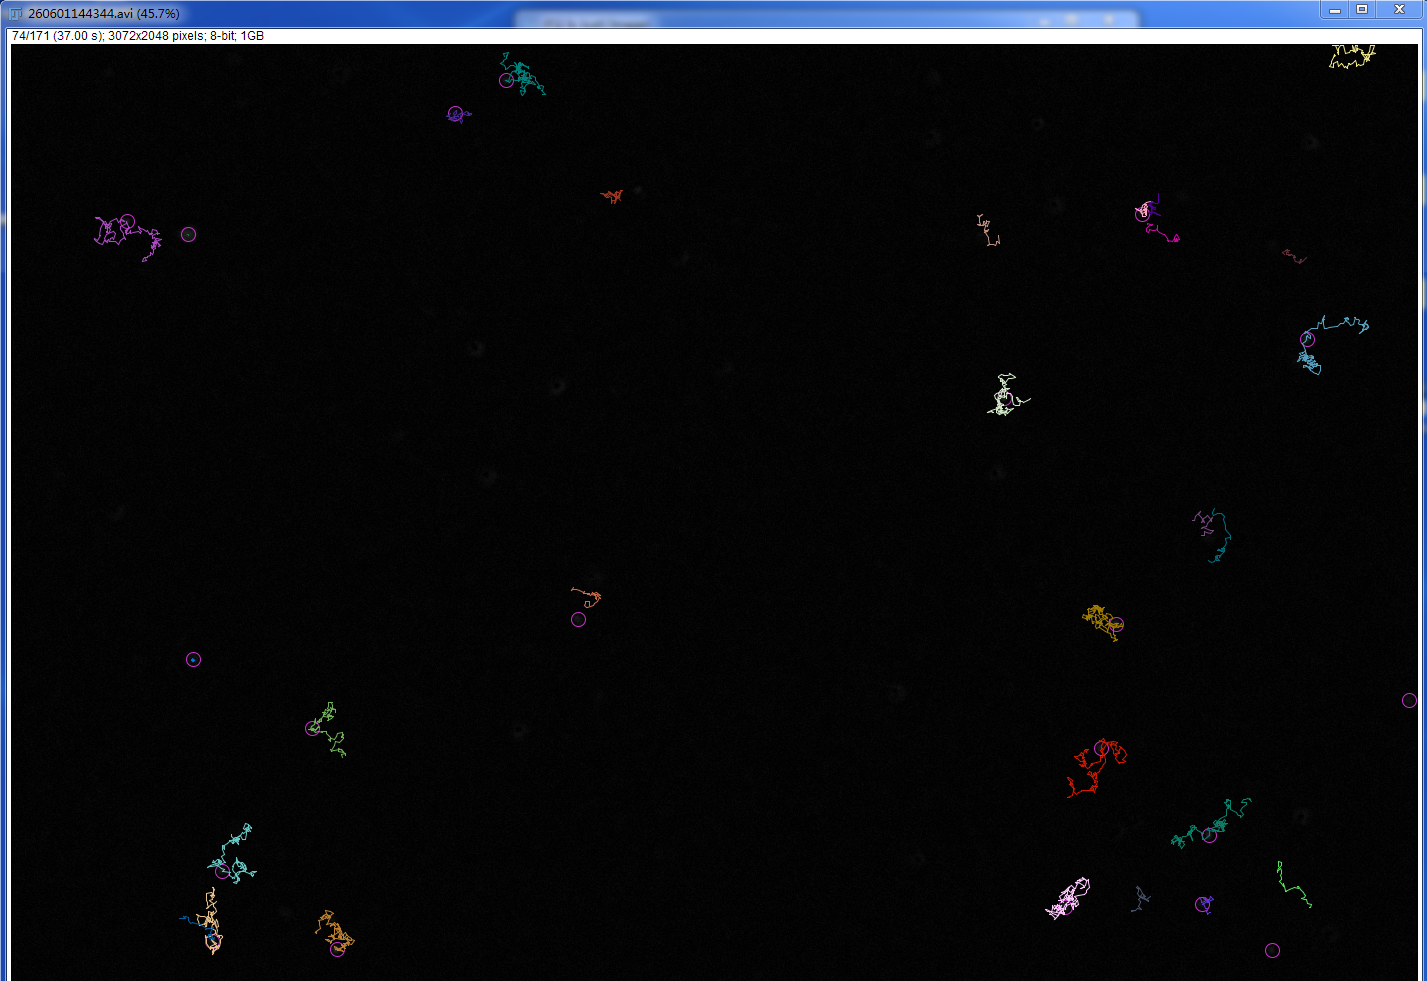
\includegraphics[width=\textwidth]{fig1.png}
        \caption{第一次实验}
    \end{subfigure}
    \hfill
    \begin{subfigure}{0.48\textwidth}
        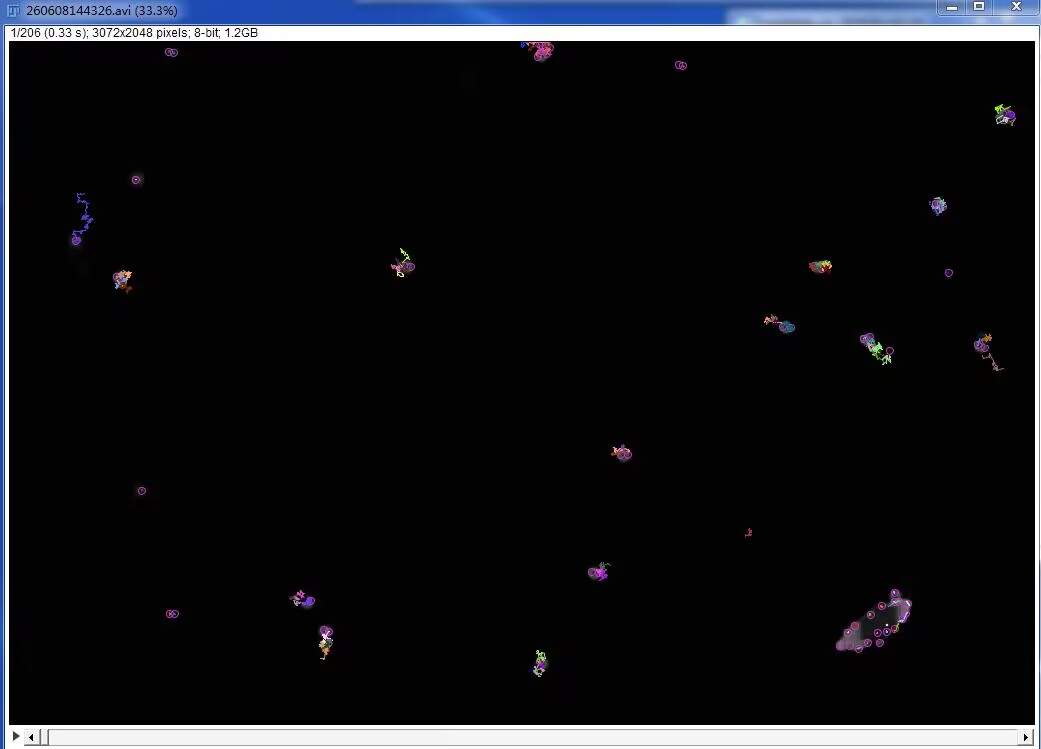
\includegraphics[width=\textwidth]{fig2.jpg}
        \caption{第二次实验}
    \end{subfigure}
    \caption{第一、二次实验的 TrackMate 轨迹}
\end{figure}

\begin{figure}[H]
    \centering
    \begin{subfigure}{0.48\textwidth}
        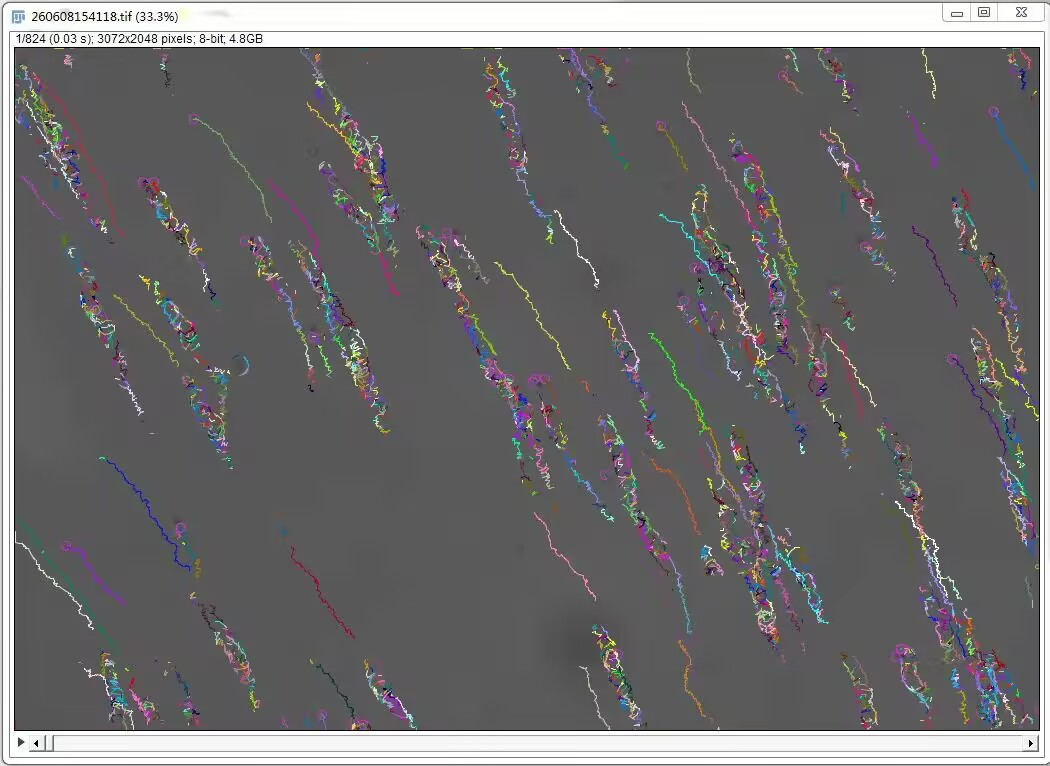
\includegraphics[width=\textwidth]{fig3.jpg}
        \caption{第三组实验第一次测量}
    \end{subfigure}
    \hfill
    \begin{subfigure}{0.48\textwidth}
        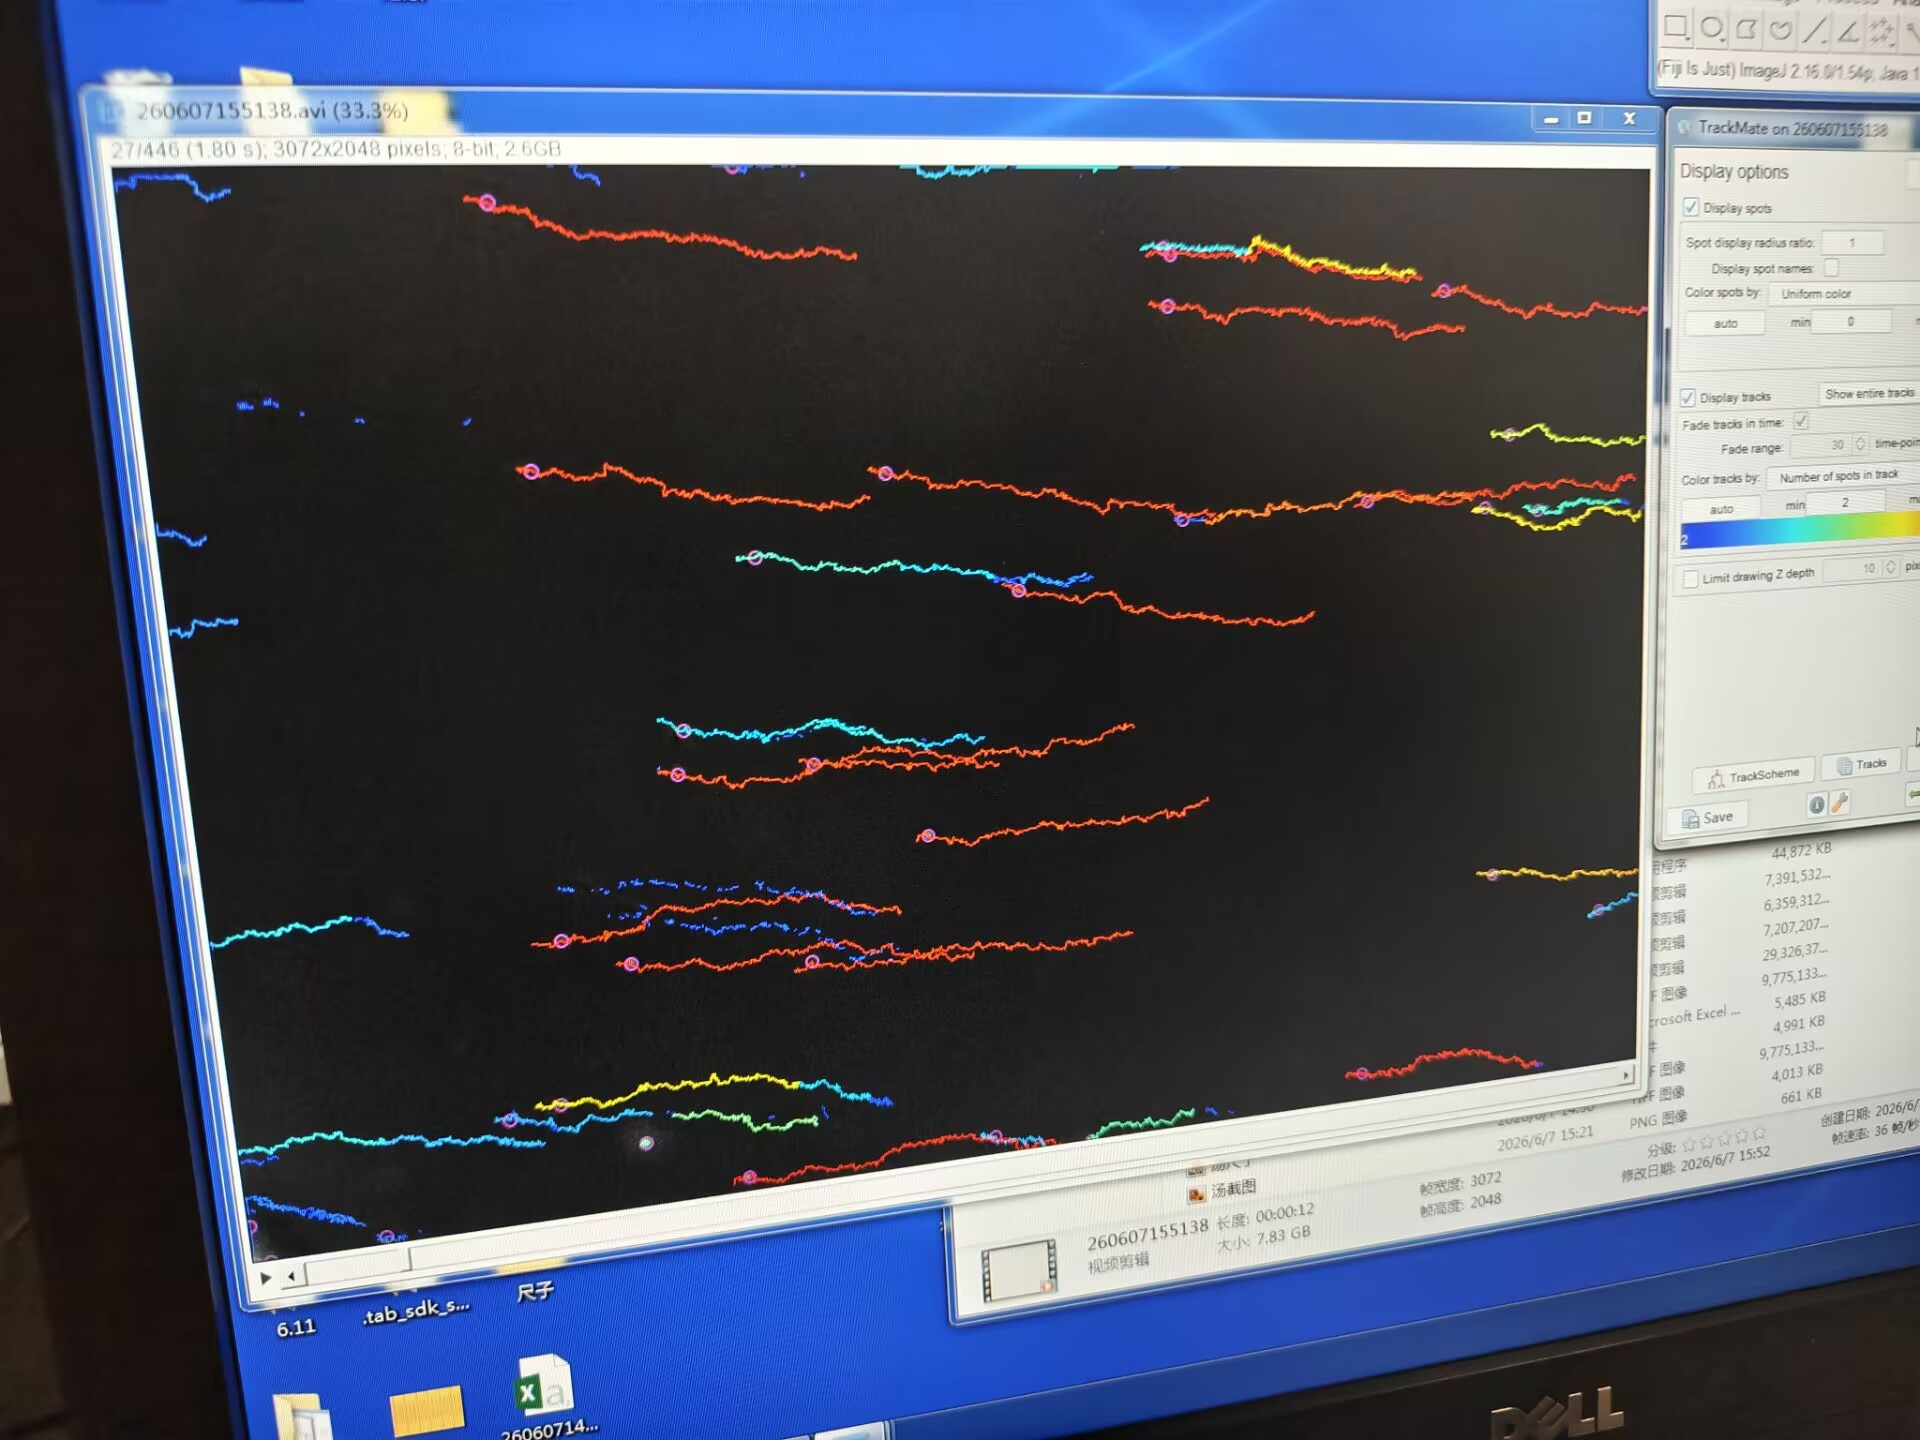
\includegraphics[width=\textwidth]{fig4.jpg}
        \caption{第三组实验第二次测量}
    \end{subfigure}
    \caption{甘油--水混合液中的两次平行测量。第一次测量具有显著同向运动，提示宏观漂移较强}
\end{figure}

\subsection{MSD 拟合与漂移修正}

\begin{table}[H]
    \centering
    \caption{未经修正与去漂移后的 MSD 拟合结果}
    \begin{tabular}{llrrrr}
        \toprule
        数据 & 处理 & 轨迹数 & $4D$（\si{\micro m^2/s}） & $D$（\si{\micro m^2/s}） & $R^2$\\
        \midrule
        1st & 原始 & 39 & 1.1502 & 0.2875 & 0.9999\\
        1st & 去漂移 & 39 & 1.0614 & 0.2654 & 0.9999\\
        2nd & 原始 & 187 & 0.1407 & 0.03517 & 0.9099\\
        2nd & 去漂移 & 187 & 0.1430 & 0.03575 & 0.9219\\
        第三组第一次 & 原始 & 402 & 4.6719 & 1.1680 & 0.9752\\
        第三组第一次 & 去漂移 & 402 & 0.7955 & 0.1989 & 0.9894\\
        第三组第二次 & 原始 & 73 & 2.8578 & 0.7145 & 0.9704\\
        第三组第二次 & 去漂移 & 73 & 0.7955 & 0.1989 & 0.9987\\
        \bottomrule
    \end{tabular}
\end{table}

\begin{figure}[H]
    \centering
    \begin{subfigure}{0.48\textwidth}
        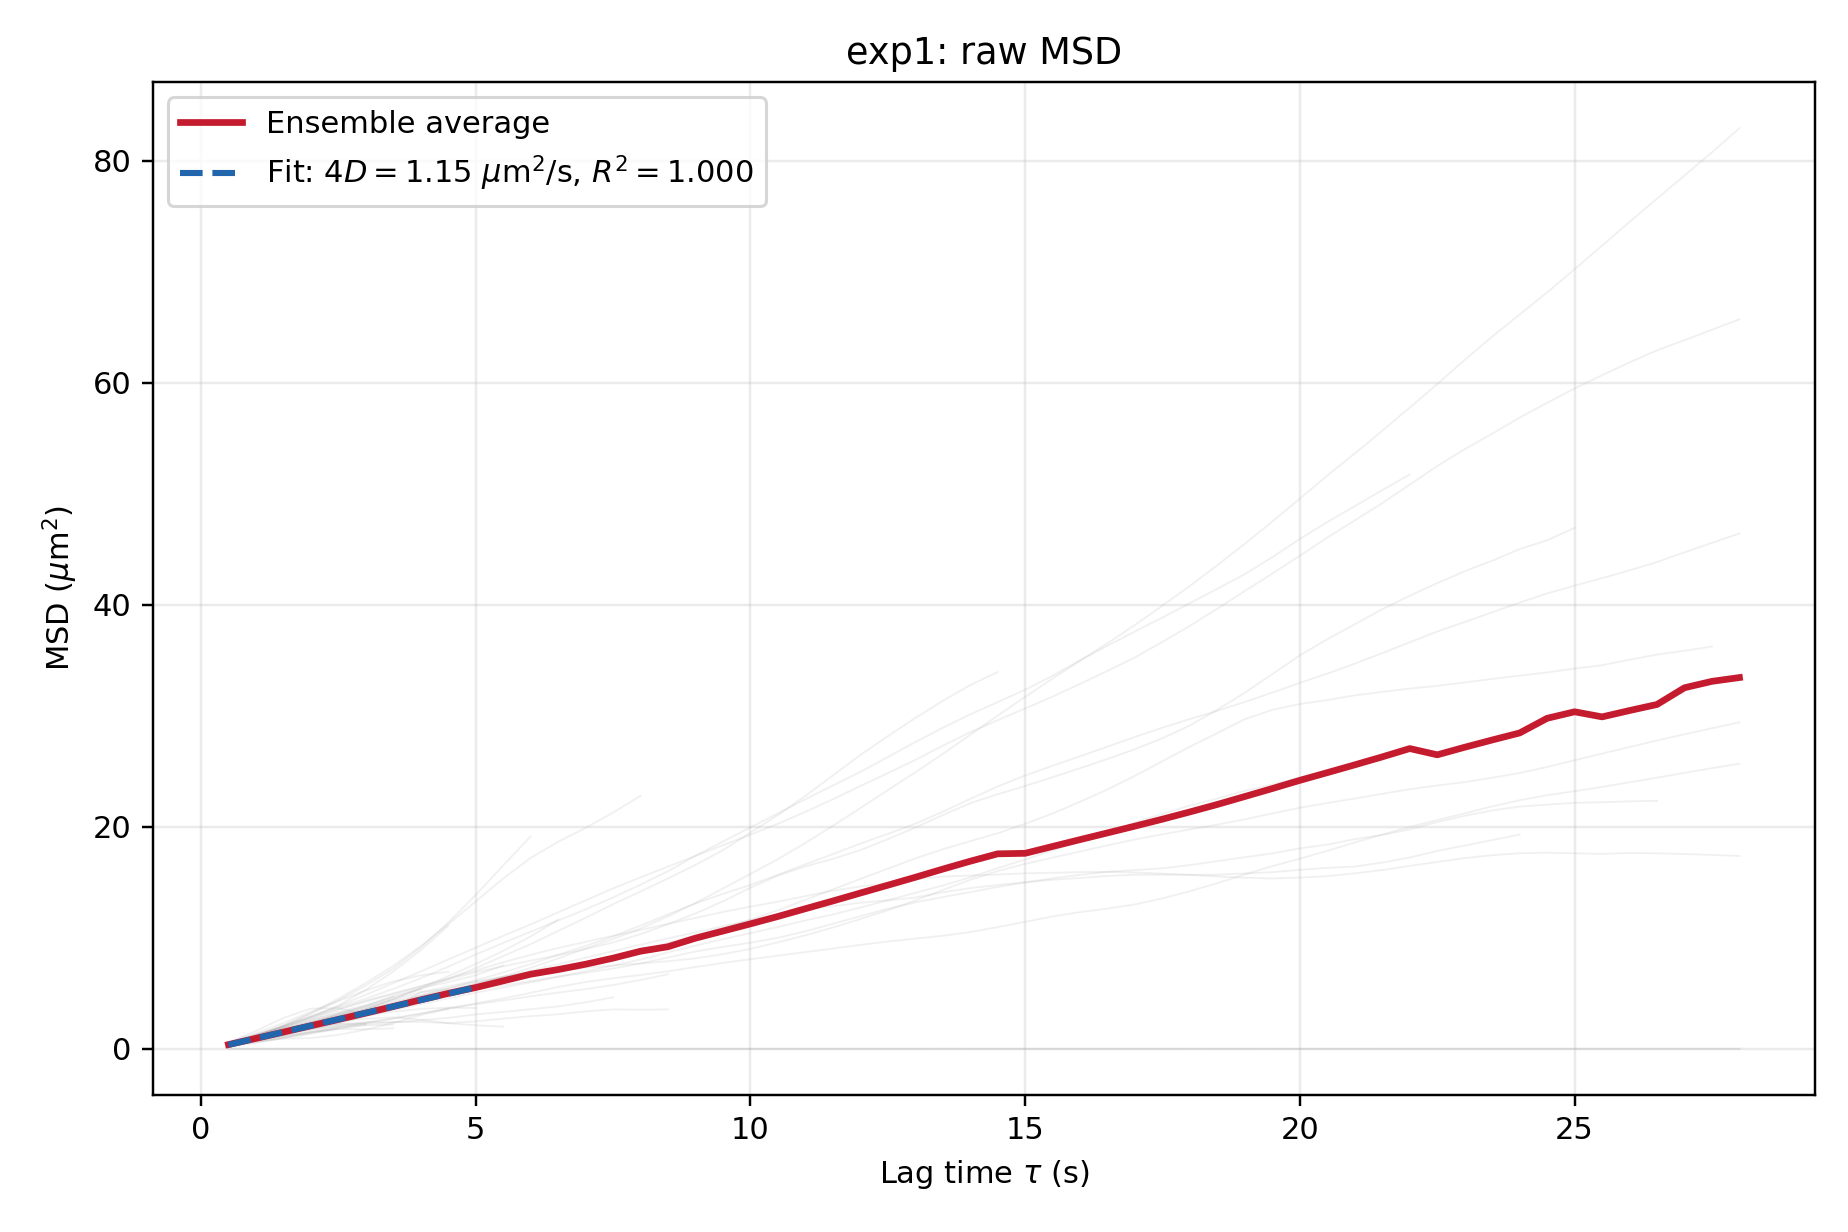
\includegraphics[width=\textwidth]{exp1_raw_msd.png}
        \caption{1st：原始}
    \end{subfigure}
    \hfill
    \begin{subfigure}{0.48\textwidth}
        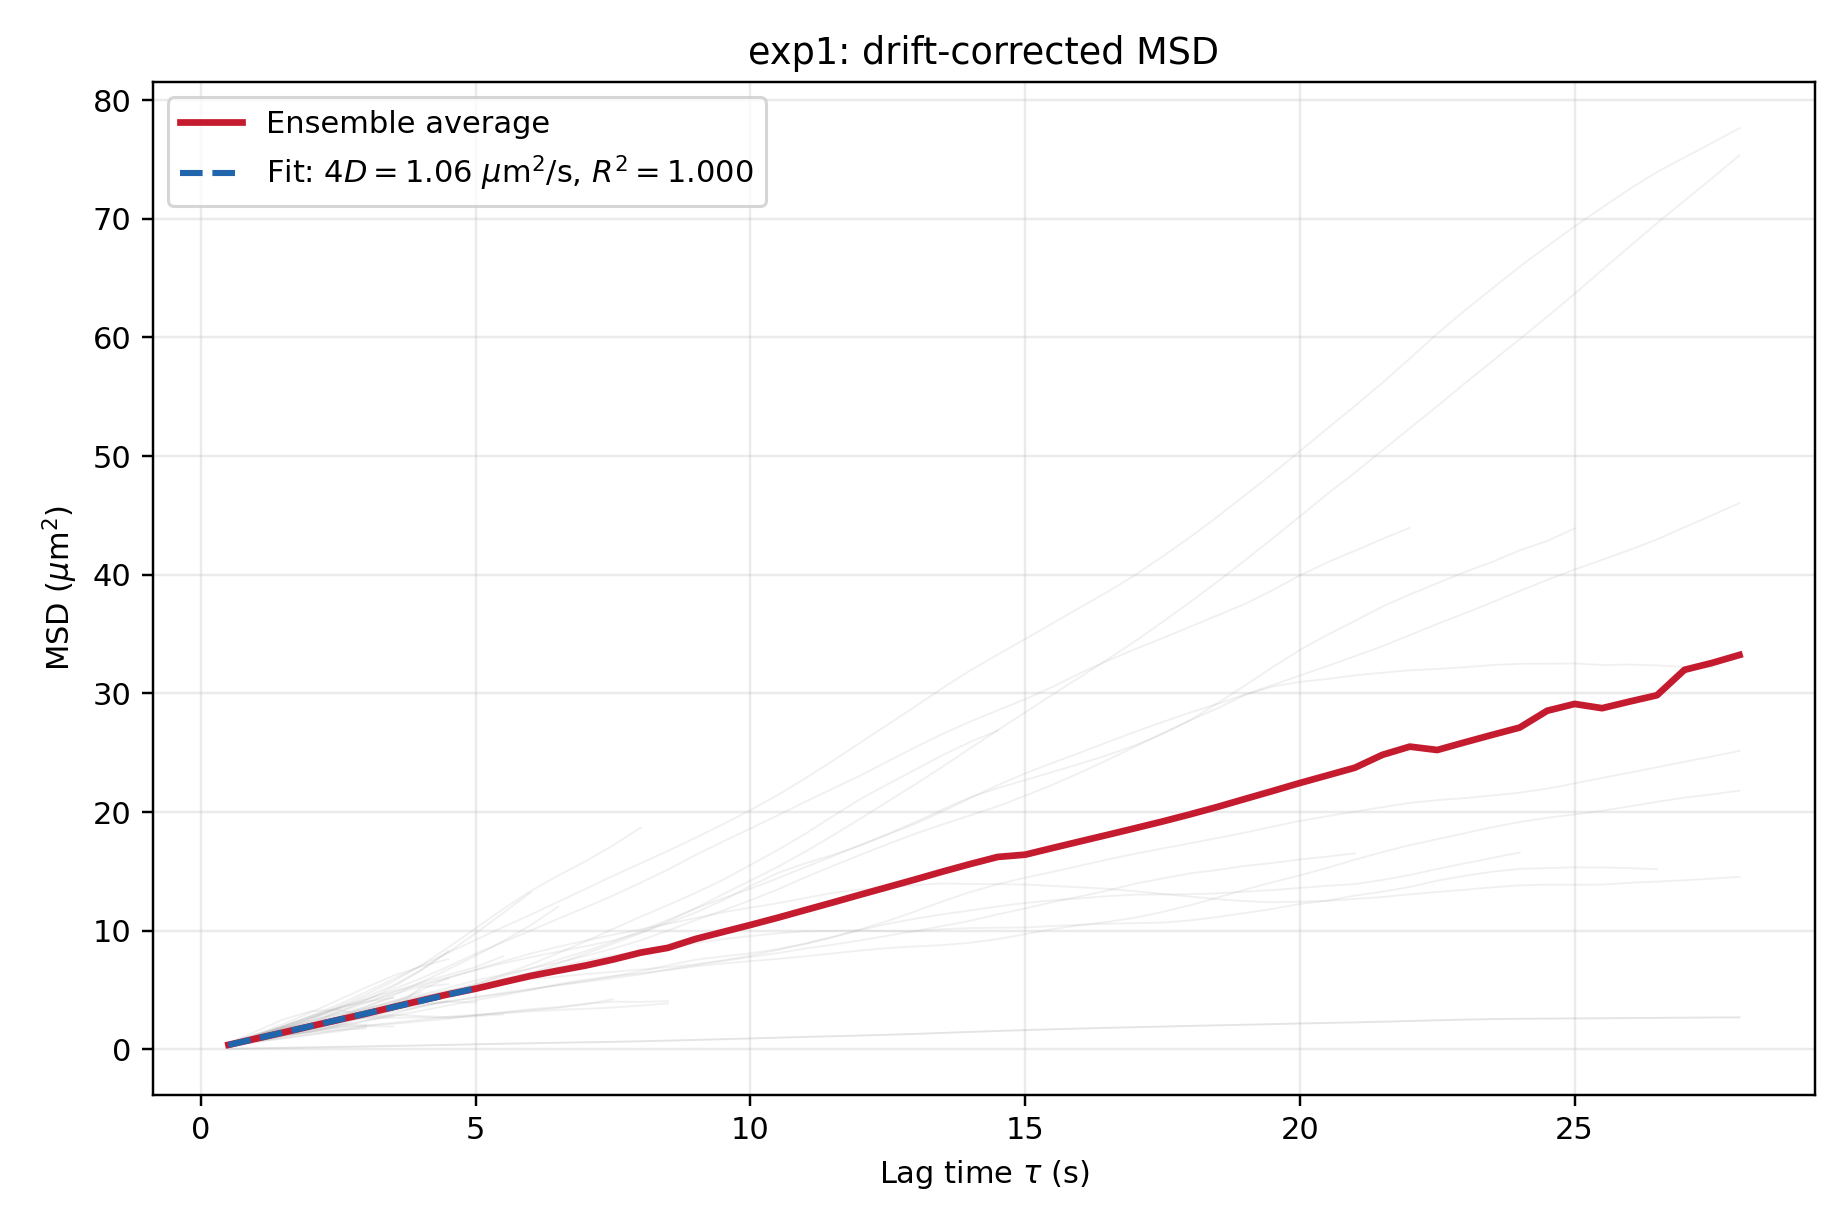
\includegraphics[width=\textwidth]{exp1_corrected_msd.png}
        \caption{1st：去漂移}
    \end{subfigure}
    \caption{第一次实验的 MSD。漂移修正使 $D$ 下降约 $7.7\%$}
\end{figure}

\begin{figure}[H]
    \centering
    \begin{subfigure}{0.48\textwidth}
        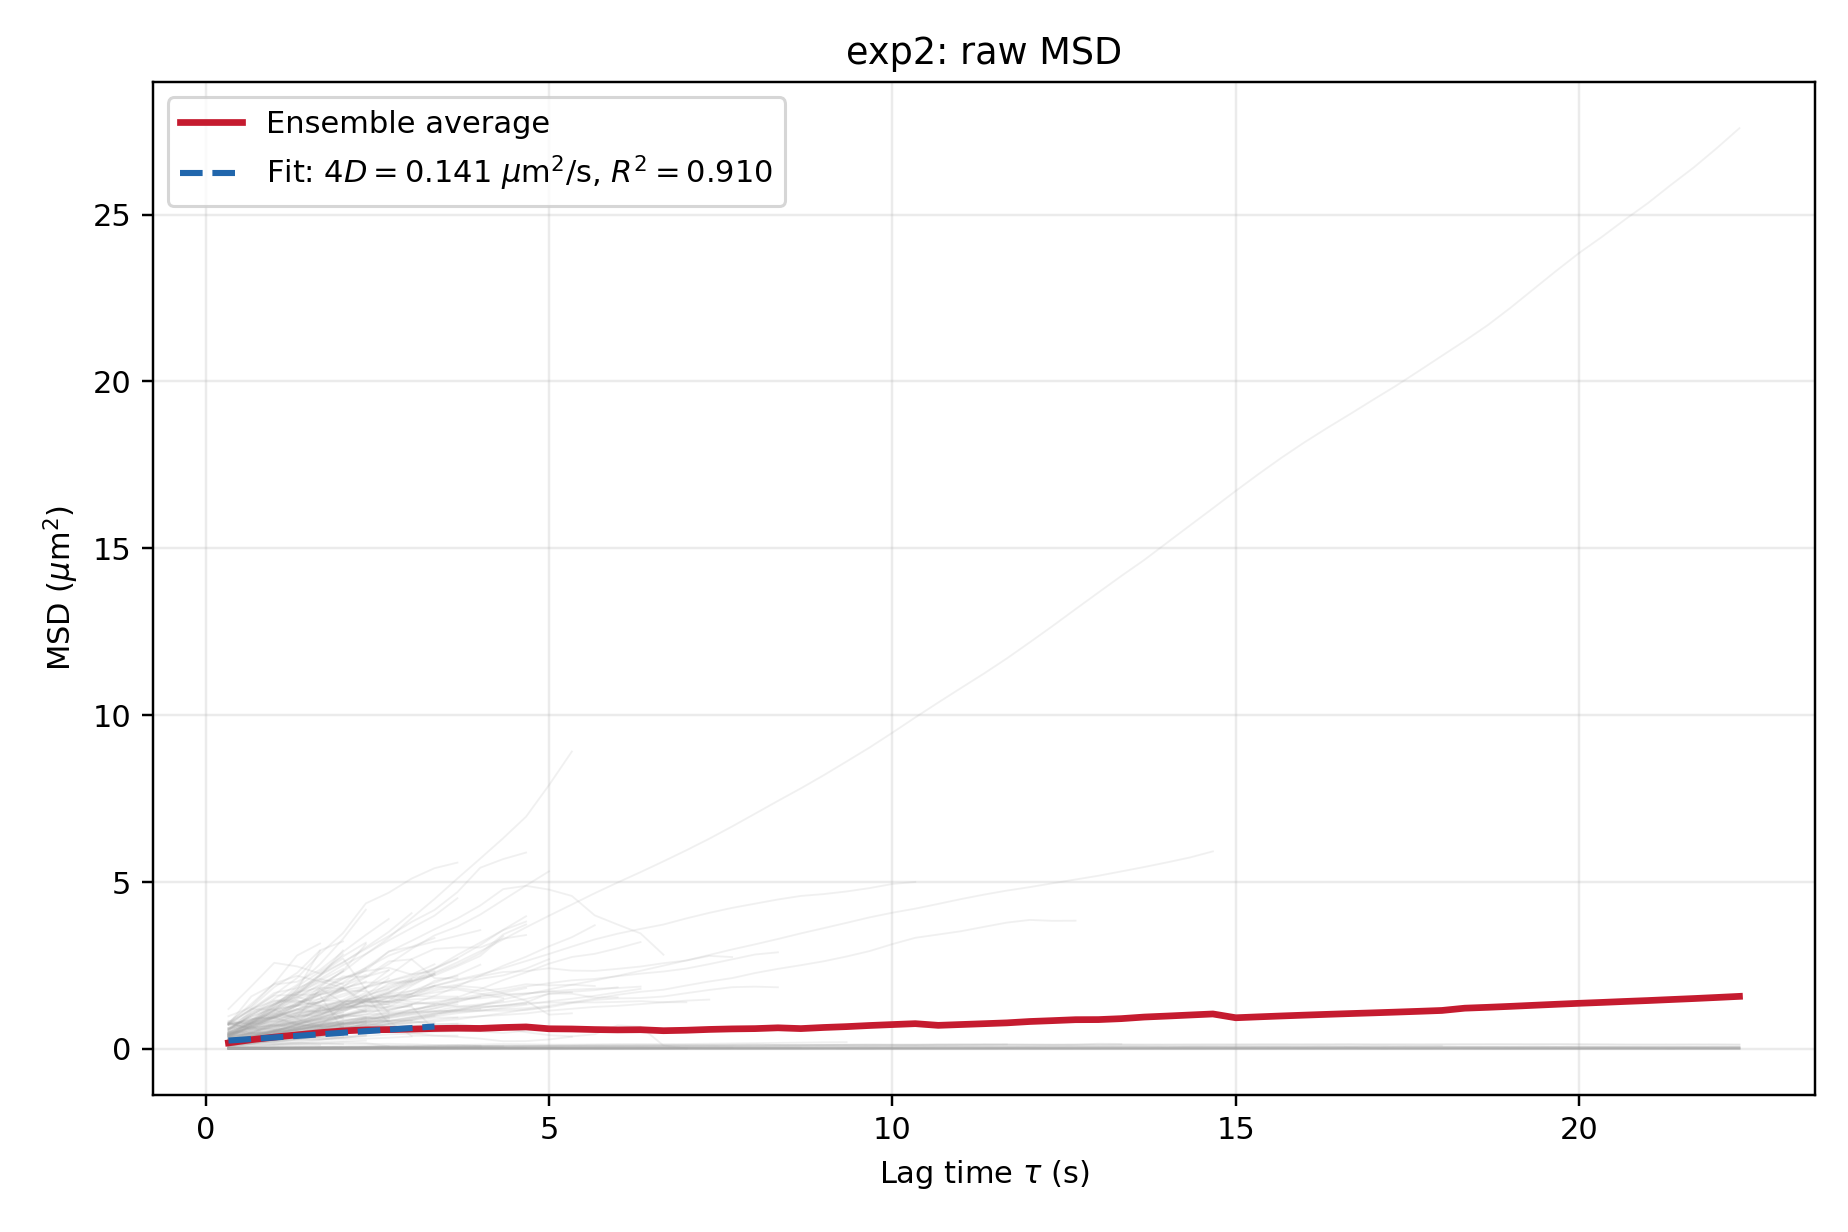
\includegraphics[width=\textwidth]{exp2_raw_msd.png}
        \caption{2nd：原始}
    \end{subfigure}
    \hfill
    \begin{subfigure}{0.48\textwidth}
        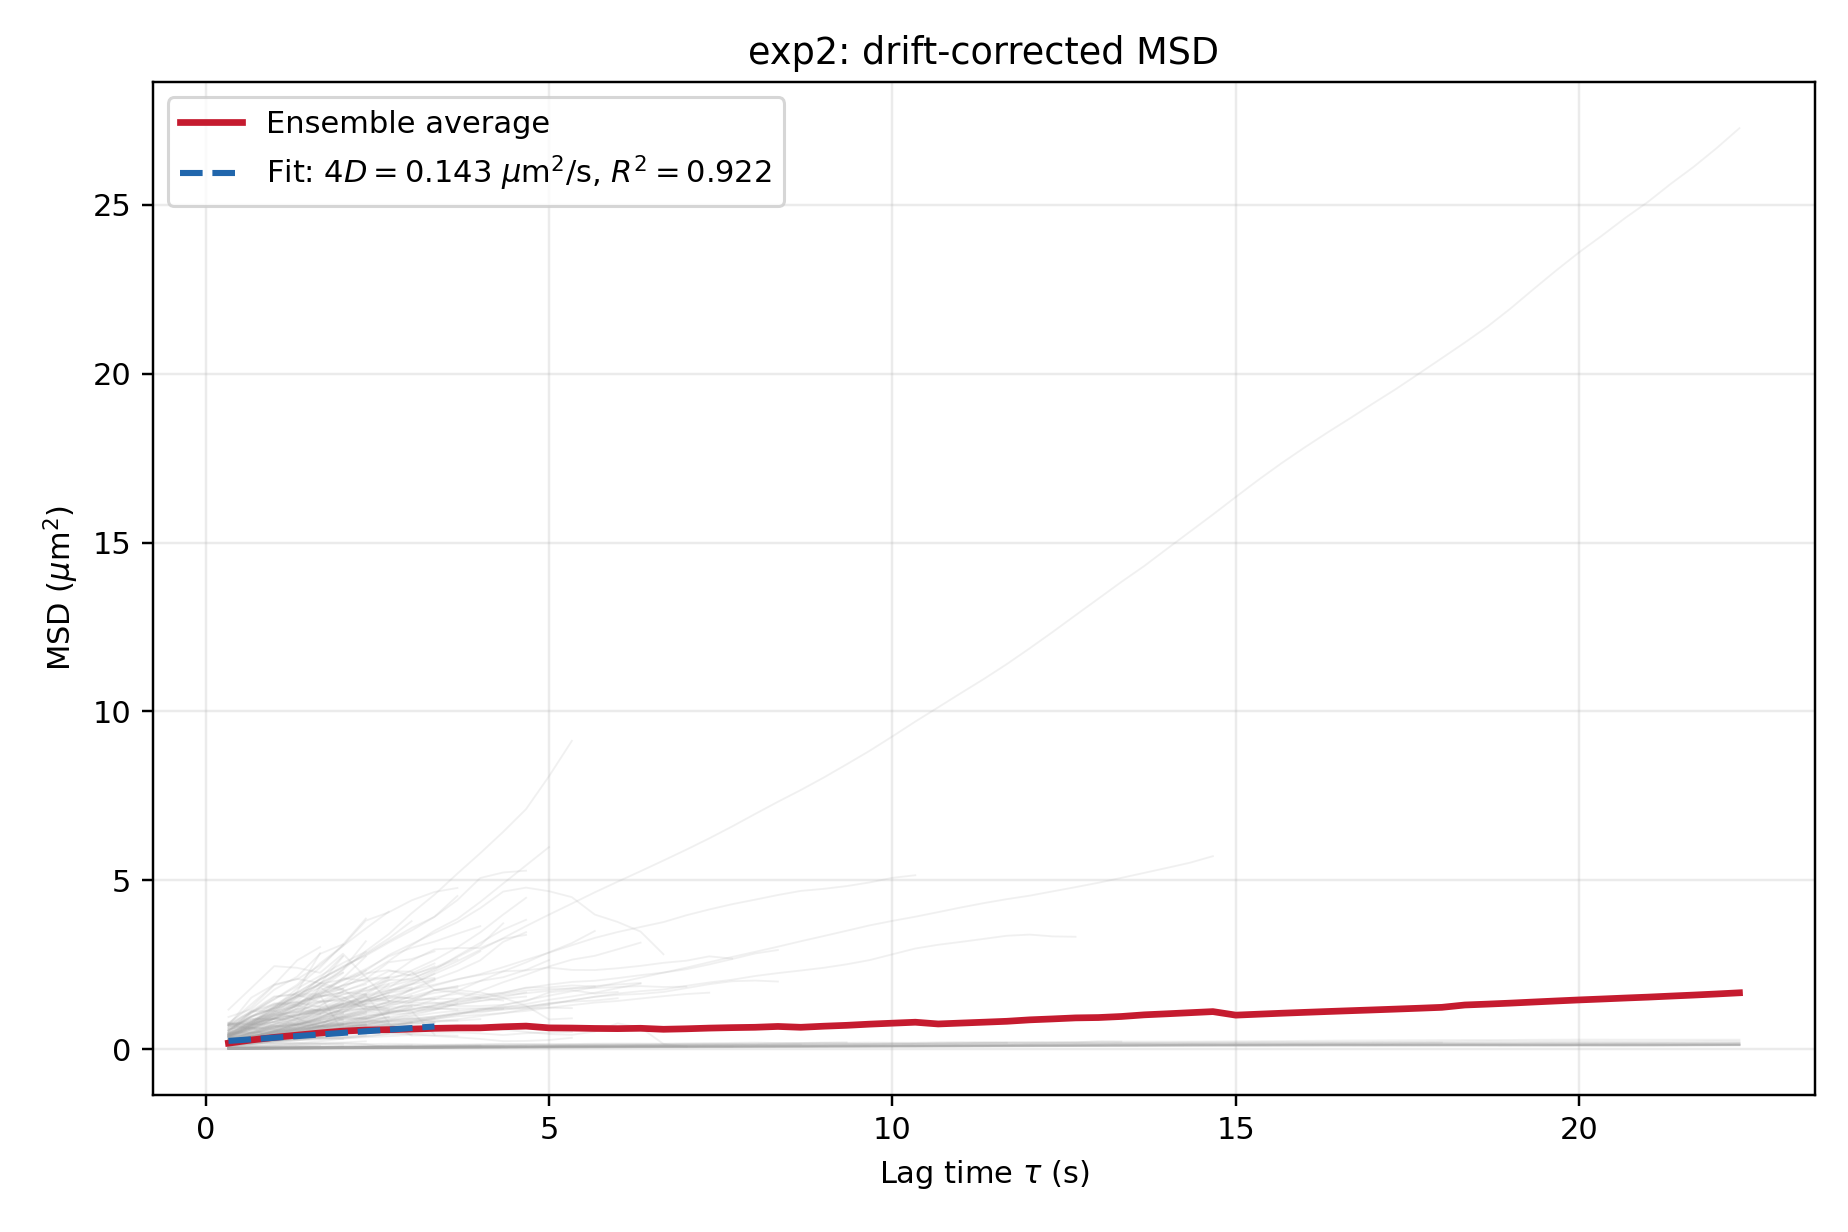
\includegraphics[width=\textwidth]{exp2_corrected_msd.png}
        \caption{2nd：去漂移}
    \end{subfigure}
    \caption{第二次实验的 MSD。修正前后结果接近，说明整体漂移较弱}
\end{figure}

\begin{figure}[H]
    \centering
    \begin{subfigure}{0.48\textwidth}
        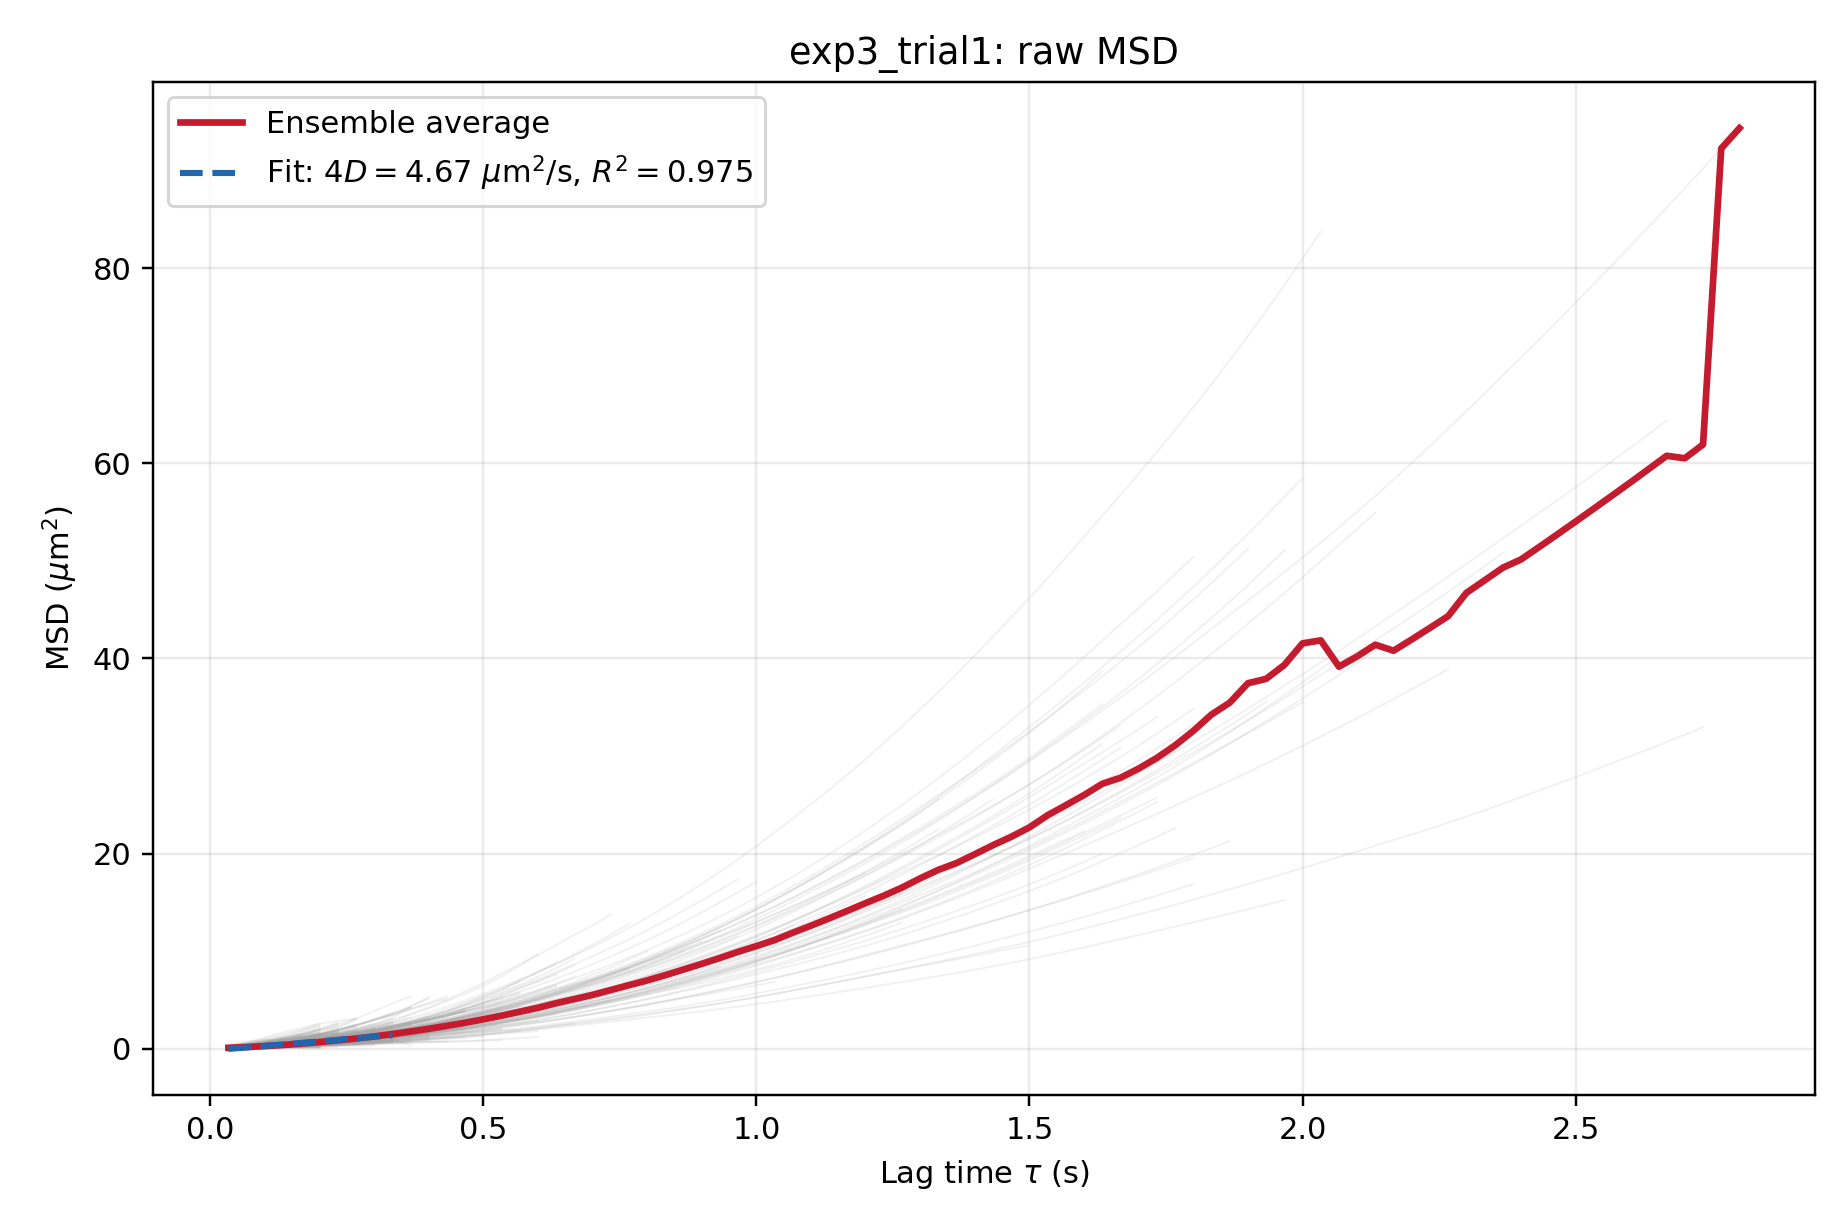
\includegraphics[width=\textwidth]{exp3_trial1_raw_msd.png}
        \caption{第一次测量：原始}
    \end{subfigure}
    \hfill
    \begin{subfigure}{0.48\textwidth}
        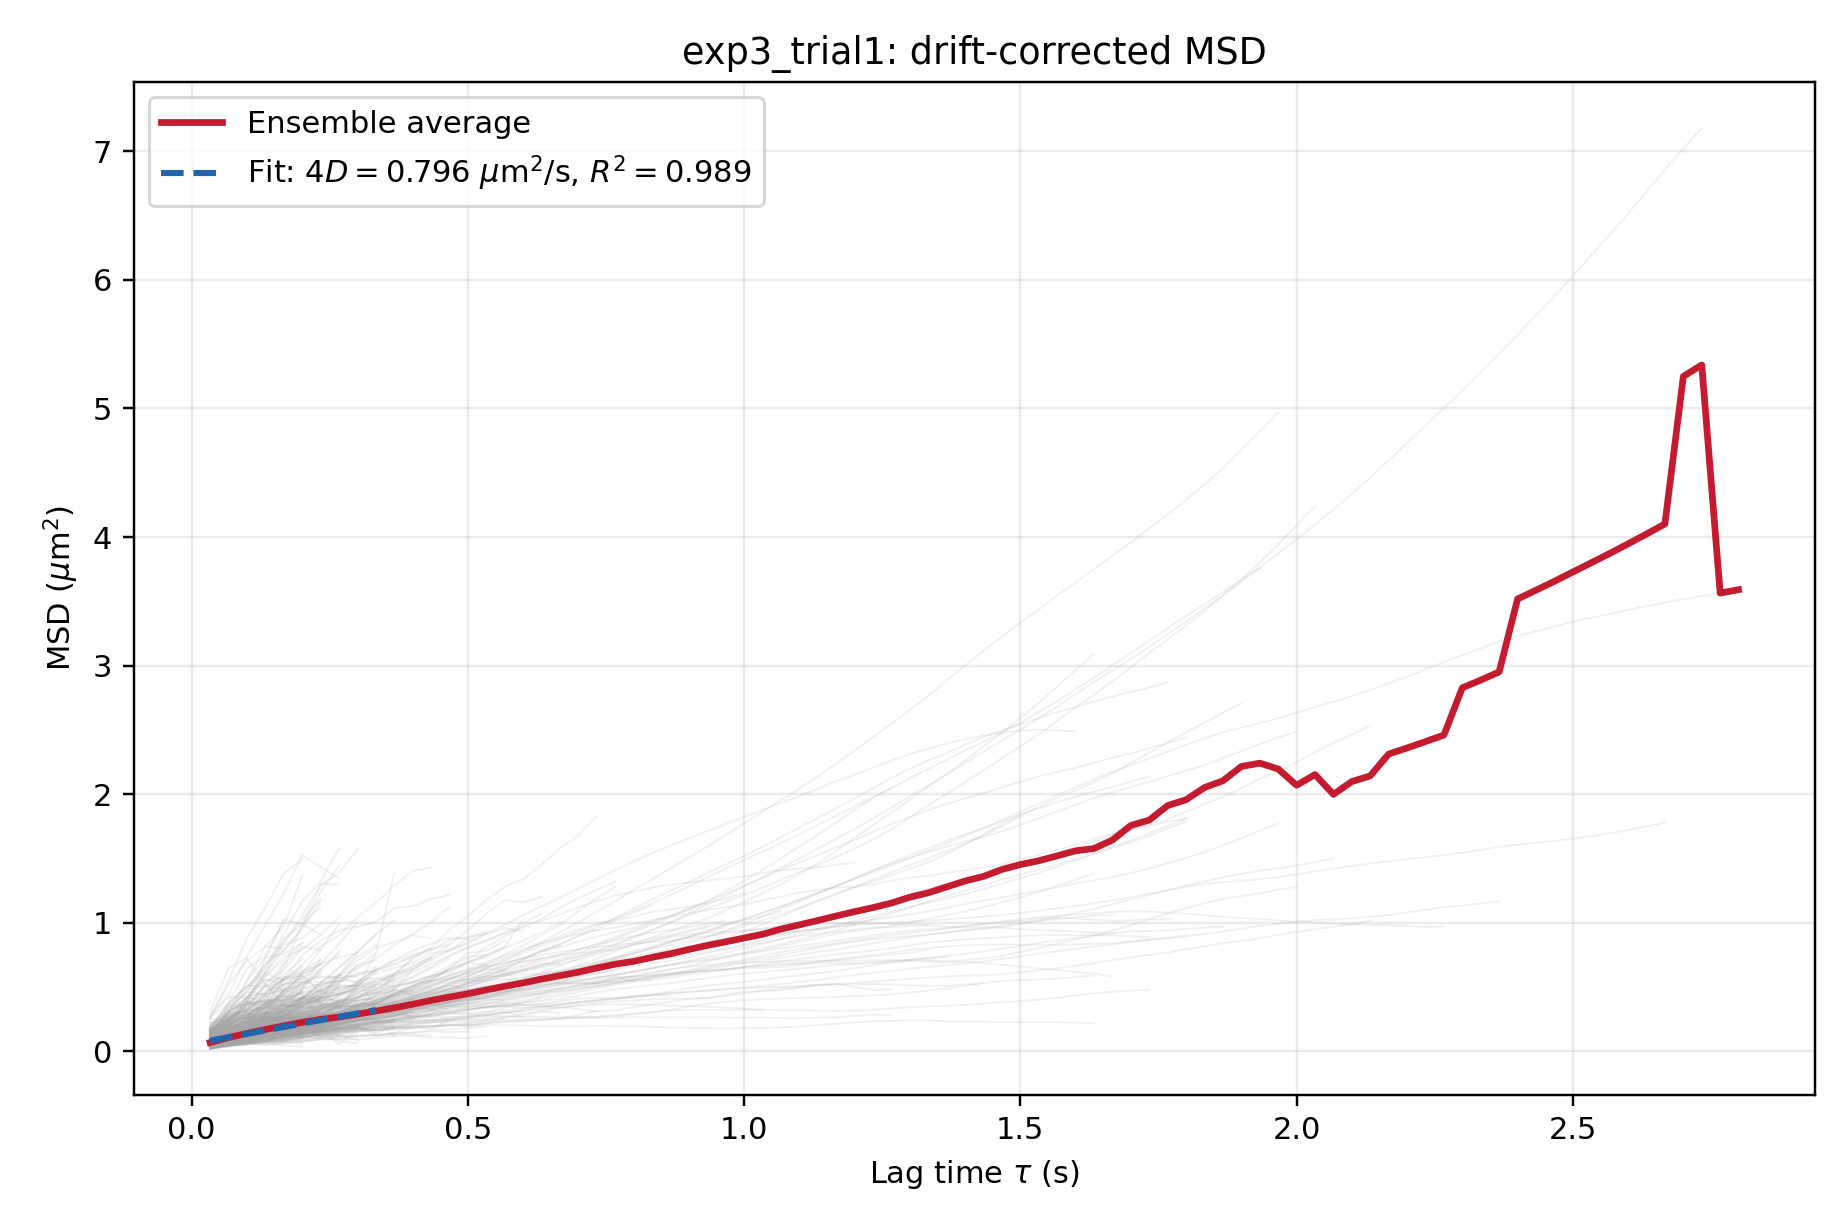
\includegraphics[width=\textwidth]{exp3_trial1_corrected_msd.png}
        \caption{第一次测量：去漂移}
    \end{subfigure}
    \caption{第三组实验第一次测量。去漂移后扩散系数降低约 $83.0\%$}
\end{figure}

\begin{figure}[H]
    \centering
    \begin{subfigure}{0.48\textwidth}
        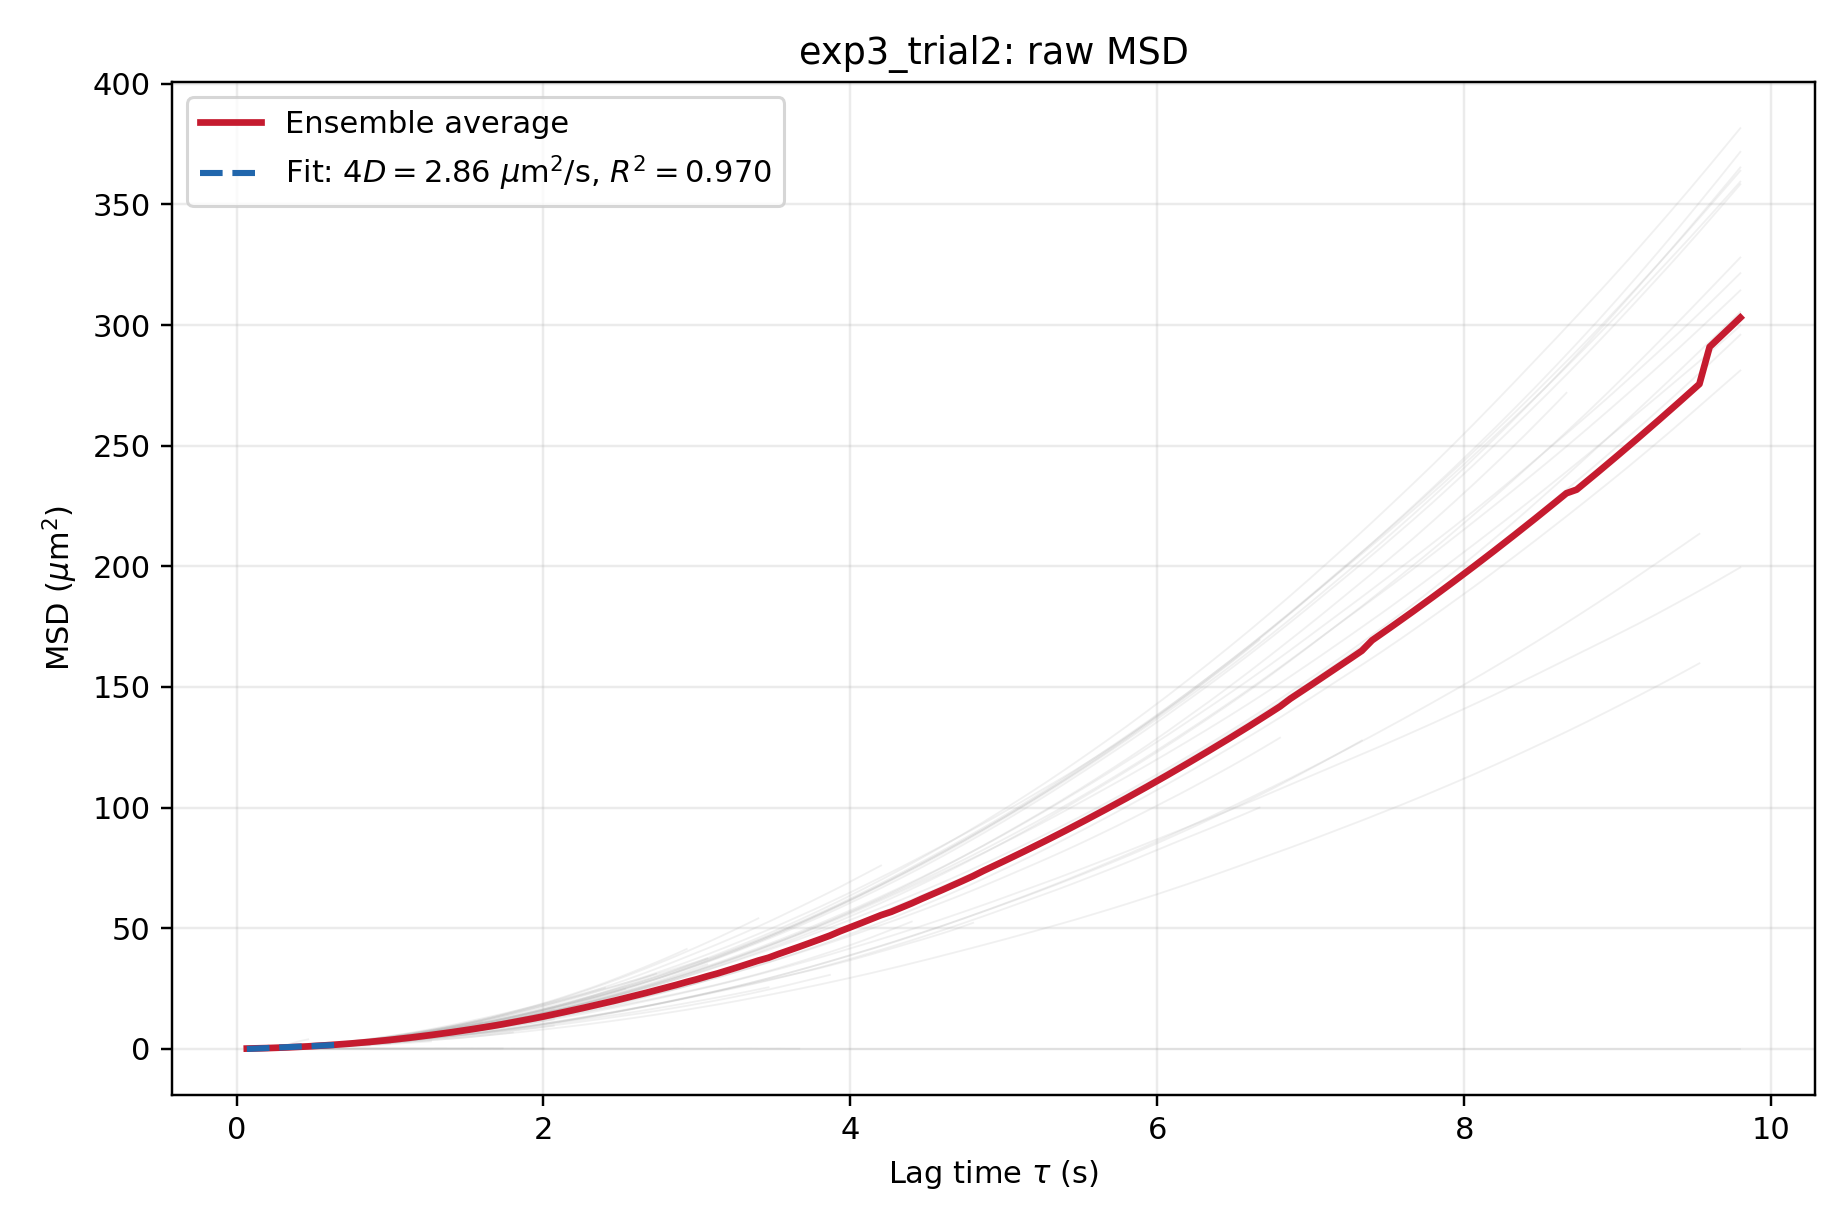
\includegraphics[width=\textwidth]{exp3_trial2_raw_msd.png}
        \caption{第二次测量：原始}
    \end{subfigure}
    \hfill
    \begin{subfigure}{0.48\textwidth}
        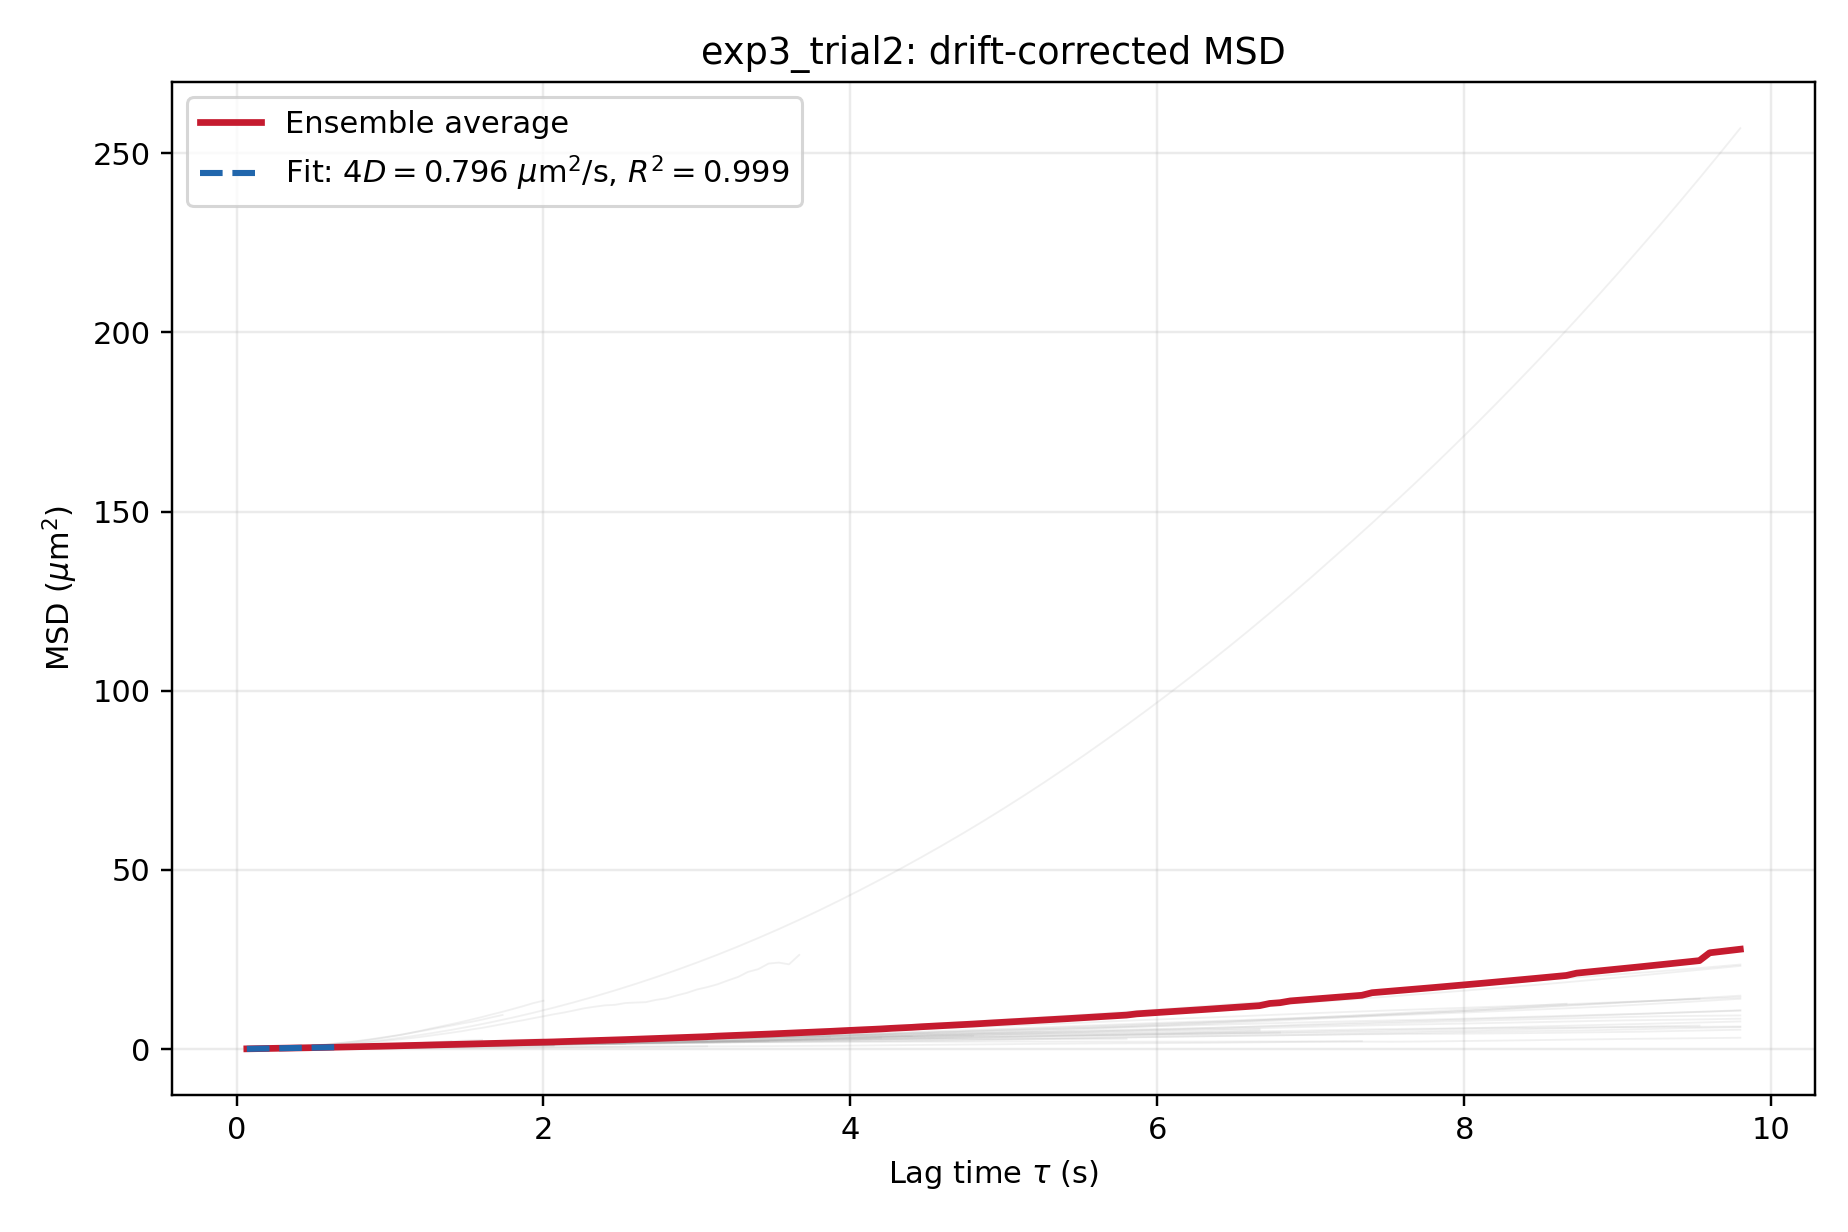
\includegraphics[width=\textwidth]{exp3_trial2_corrected_msd.png}
        \caption{第二次测量：去漂移}
    \end{subfigure}
    \caption{第三组实验第二次测量。去漂移后扩散系数降低约 $72.2\%$}
\end{figure}

\subsubsection{拟合参数的物理含义}

理想二维布朗运动的 MSD 应通过原点，但真实实验更适合写成
\begin{equation}
    \mathrm{MSD}_{\mathrm{obs}}(\tau)
    =4D\tau+4\sigma_{\mathrm{loc}}^2+v^2\tau^2+\varepsilon(\tau),
    \label{eq:realmsd}
\end{equation}
其中 $\sigma_{\mathrm{loc}}$ 是单坐标定位误差，$v$ 是未消除的平均漂移速度，
$\varepsilon(\tau)$ 包含有限样本涨落、轨迹连接误差和非均匀流动。因而：
\begin{itemize}
    \item 短延迟区斜率主要给出 $4D$；
    \item 正截距主要来自定位误差，近似有 $\sigma_{\mathrm{loc}}\approx\sqrt{b/4}$；
    \item 长延迟区向上弯曲通常对应 $v^2\tau^2$ 或对流；
    \item 长延迟区下凹则可能来自受限扩散、壁面束缚、有限视野筛选或运动模糊。
\end{itemize}
本文只取最早 10 个延迟点拟合，是为了在保留足够位移统计的同时，尽量避开长时间尺度上的对流和有限视野效应。表中 $R^2$ 衡量的是所选短时区间内的线性程度，并不能单独证明整个时间范围均为理想扩散。

\subsubsection{各组曲线的比较}

第一次实验修正前后 $D$ 从 \SI{0.2875}{\micro m^2/s} 变为
\SI{0.2654}{\micro m^2/s}，变化为 $7.7\%$。短时线性拟合的
$R^2=0.9999$，斜率标准误对应
$D=\SI{0.2654(11)}{\micro m^2/s}$。这说明该组在拟合区间内最接近正常扩散。
其拟合截距略为负值，不应解释成“负定位误差”，而是说明截距与斜率在有限拟合区间内存在相关性，同时有限曝光会压低最短延迟处的 MSD。

第二次实验的去漂移结果为
$D=\SI{0.03575(368)}{\micro m^2/s}$，相对拟合不确定度约为 $10.3\%$，
明显高于第一次实验。其正截距
$b=\SI{0.195}{\micro m^2}$ 对应等效单坐标定位误差
$\sigma_{\mathrm{loc}}\approx\SI{0.221}{\micro m}$。当真实布朗位移较小时，定位噪声在总 MSD 中所占比例增大，导致 $R^2$ 下降。修正前后 $D$ 仅变化约 $1.6\%$，说明这一组的主要限制不是整体平移，而是定位分辨率、轨迹连接和较弱扩散信号之间的竞争。

第三组实验第一次测量的原始轨迹呈明显同向延伸。采用各自有效标定后，两次测量的结果为
\begin{align}
    D_{\mathrm{u},1}^{\mathrm{raw}}&=\SI{1.168}{\micro m^2/s},&
    D_{\mathrm{u},1}&=\SI{0.1989(73)}{\micro m^2/s},\\
    D_{\mathrm{u},2}^{\mathrm{raw}}&=\SI{0.7145}{\micro m^2/s},&
    D_{\mathrm{u},2}&=\SI{0.1989(26)}{\micro m^2/s}.
\end{align}
若将原始曲线前 25 个延迟点近似拟合为
$4D\tau+v^2\tau^2+b$，二次项给出的等效漂移速度约为
\SI{3.03}{\micro m/s}。第二次测量对应的等效漂移速度约为
\SI{1.74}{\micro m/s}。去漂移后两次扩散系数一致，说明分别处理视频尺度后，
两次独立轨迹给出了相互一致的热扩散量级。

去漂移后，第三组第一次测量仍有
$b=\SI{0.0577}{\micro m^2}$，对应
$\sigma_{\mathrm{loc}}\approx\SI{0.120}{\micro m}$；第二次测量截距接近零。
这表明两次视频在图像对比度、焦面、粒子尺寸分布或轨迹识别质量上并不完全等价。
此外，质心法只能消除空间上近似均匀的平移流；若速度随位置变化（剪切流）或随时间变化，
不同粒子会经历不同的确定性位移，修正后的 MSD 中仍会保留非布朗贡献。

\subsection{第一次实验：玻尔兹曼常数}

第一、三组粒子的标称直径范围为
$d_1=0.6$--\SI{1.0}{\micro m}。代入去漂移后的
$D_1=\SI{0.2654}{\micro m^2/s}$ 可得
\begin{equation}
    k_B=\left(\SI{7.72e-24}{J.K^{-1}}\right)
    \left(\frac{d_1}{\si{\micro m}}\right).
\end{equation}
因此实验值范围为
\begin{equation}
    k_B=(4.63\text{--}7.72)\times10^{-24}\ \si{J.K^{-1}}.
\end{equation}
与理论值 \SI{1.380649e-23}{J.K^{-1}} 比较，相对偏差范围为
\begin{equation}
    \frac{|k_B-k_{B,0}|}{k_{B,0}}
    =44.1\%\sim66.5\%.
\end{equation}
若取标称范围中值 $d_1=\SI{0.8}{\micro m}$，则
$k_B=\SI{6.17e-24}{J.K^{-1}}$，相对误差为 $55.3\%$。
实验值系统性偏低，说明除粒径分布外，比例尺、运动模糊、近壁阻力和轨迹筛选均可能使
测得的扩散系数偏小。

\subsection{第二次实验：改变粒径}

第二次实验去漂移后的扩散系数为
$D_2=\SI{0.03575}{\micro m^2/s}$。若两次均为同温度纯水且只改变粒径，则
\begin{equation}
    \frac{d_2}{d_1}=\frac{D_1}{D_2}=7.42.
\end{equation}
结合 $d_1=0.6$--\SI{1.0}{\micro m}，得到第二组粒径范围
\begin{equation}
    d_2=4.45\text{--}7.42\ \si{\micro m}.
\end{equation}
结果在方向上符合 $D\propto 1/d$：较大粒子扩散显著变慢。
由于第二组粒子的厂家标称直径仍未知，尚不能计算第二组粒径的相对误差。
需要注意，若两组视频确实使用完全相同的光学倍率和比例尺，
比值 $D_1/D_2$ 中共同的 $s^2$ 会抵消；但两次帧率、焦面、壁面距离或样品黏度的差异不会抵消。
第二次实验较大的相对拟合误差也会直接传递到直径比中。

\subsection{第三次实验：甘油--水混合液黏度}

第三组实验与第一组使用同一种粒子，且温度相同，因此粒径和 $k_B$ 在比值中消去。两次测量结果分别为
\begin{align}
    \eta_{\mathrm{u},1}
    &=\eta_{\mathrm w}\frac{D_1}{D_{\mathrm{u},1}}
      =\SI{1.222}{mPa.s},\\
    \eta_{\mathrm{u},2}
    &=\eta_{\mathrm w}\frac{D_1}{D_{\mathrm{u},2}}
      =\SI{1.222}{mPa.s}.
\end{align}
两组算术平均为
\begin{equation}
    \bar{\eta}_{\mathrm u}=\SI{1.222}{mPa.s}.
\end{equation}
该值比同温度纯水的 \SI{0.916}{mPa.s} 高约 $33.4\%$，与加入少量甘油后液体黏度上升的物理预期一致。
两次视频在原始像素坐标下给出的扩散量级不同，但在分别采用有效比例尺并去除共同漂移后结果吻合，
说明原始差异主要来自视频尺度和宏观流动，而非液体本征黏度发生变化。

\subsection{误差分析}

\begin{enumerate}
    \item \textbf{空间比例尺的平方传播。}
    实际坐标为 $\bm r=s\bm r_{\mathrm{px}}$，所以
    $\mathrm{MSD}=s^2\mathrm{MSD}_{\mathrm{px}}$、$D\propto s^2$。一阶误差传播为
    \begin{equation}
        \frac{\delta D}{D}=2\frac{\delta s}{s}.
    \end{equation}
    第一、二组采用 \SI{0.100}{\micro m/pixel}，第三组两次视频分别采用
    \SI{0.0551}{\micro m/pixel} 和 \SI{0.0762}{\micro m/pixel}。
    不同视频的倍率与缩放不同，若强行使用同一比例尺，会造成显著系统差异。
    对 $k_B$ 有 $k_B\propto s^2$；只有参考组与待测组采用同一有效标定时，
    黏度比值中的公共 $s^2$ 才能严格抵消。

    \item \textbf{时间轴、丢帧与有限曝光。}
    由 $\tau=m/f$ 可知 $D\propto f$，因此
    $\delta D/D=\delta f/f$。本文帧率由截图读取，而不是从原视频元数据自动校验；
    若视频转码、抽帧或播放帧率与采集帧率不同，会造成系统偏差。
    相机在曝光时间 $t_e$ 内记录的是粒子位置的时间平均，而非瞬时位置，
    运动模糊通常压低最短延迟的 MSD，使拟合截距偏负并使斜率依赖拟合起点。

    \item \textbf{定位噪声与有限光学分辨率。}
    若每个坐标的定位噪声方差为 $\sigma_{\mathrm{loc}}^2$，两个时刻的误差相减后，
    二维 MSD 增加约 $4\sigma_{\mathrm{loc}}^2$。第二次实验的
    $\sigma_{\mathrm{loc}}$ 约为 \SI{0.22}{\micro m}，第三组第一次测量约为
    \SI{0.12}{\micro m}。当单帧真实布朗位移与此量级相近时，
    截距项会占据显著比例，斜率对拟合区间更敏感。离焦、低信噪比、粒子图像重叠及检测阈值变化
    都会改变定位精度。

    \item \textbf{宏观对流和非均匀流场。}
    恒定速度产生 $v^2\tau^2$ 项，从而把仅用直线拟合得到的 $D$ 推高。
    第三组两次测量的原始曲线给出约 \SI{3.03}{\micro m/s} 和
    \SI{1.74}{\micro m/s} 的等效漂移速度，说明对流不是小修正，而是主导系统效应。
    质心法可消除共同平移，却不能完全消除剪切流、旋涡、蒸发诱导流和随时间变化的流速。
    残余对流会使 $D$ 偏大，继而使由 $\eta\propto1/D$ 得到的黏度偏小。

    \item \textbf{近壁流体动力学修正。}
    式 \eqref{eq:se} 假设球体处于无限大连续介质。粒子中心距平面壁为 $h$ 时，
    平行于壁面的迁移率可用 Faxén 展开近似修正：
    \begin{equation}
        \frac{D_{\parallel}}{D_0}
        \approx1-\frac{9}{16}\frac{a}{h}
        +\frac{1}{8}\left(\frac{a}{h}\right)^3
        -\frac{45}{256}\left(\frac{a}{h}\right)^4+\cdots .
    \end{equation}
    因而靠近载玻片或盖玻片时 $D$ 小于体相值。若忽略该效应，反推粒径和黏度都会偏大。
    不同视频的焦面高度不同，也会造成即使粒径和液体相同，测得 $D$ 仍不一致。

    \item \textbf{粒子非理想性与样品条件。}
    Stokes--Einstein 关系默认粒子为孤立刚性球、液体为牛顿流体且无粒子间相互作用。
    实际胶体可能具有粒径分布、团聚、电荷双层作用或非球形；浓度过高时还会出现流体动力学耦合。
    温度误差同时影响显式的 $T$ 和黏度 $\eta(T)$，且水在室温附近的黏度对温度较敏感。
    第一、三组粒径只给出 $0.6$--\SI{1.0}{\micro m} 的范围，该范围本身会使
    $k_B$ 产生约 $\pm25\%$（相对于中值）的粒径不确定度；第二组粒径标称值仍缺失。

    \item \textbf{轨迹连接与选择偏差。}
    TrackMate 的最大连接距离过大会把相邻粒子误连，产生异常大步长；过小则会截断快速粒子轨迹。
    只保留不少于 20 帧的轨迹可提高统计稳定性，但也可能 preferentially 保留运动慢、离开视野较晚的粒子，
    使 $D$ 偏小。有限视野还会使快速粒子更容易消失，形成典型的存活选择偏差。

    \item \textbf{有限样本与相关位移。}
    延迟为 $m$ 帧时，一条长度为 $N$ 的轨迹只有 $N-m$ 个位移，而且这些重叠位移并非完全独立。
    因此普通线性回归给出的斜率标准误只反映拟合残差，往往低估包含轨迹间差异后的总不确定度。
    第三组两次测量经分别标定后相互一致；但尺度标定的不确定度没有包含在回归标准误中，
    因而单条平均曲线的拟合误差仍会低估总不确定度。
    更严格的方法应以粒子为单位 bootstrap，重复抽取整条轨迹后重新计算系综 MSD 和 $D$。

    \item \textbf{模型与拟合区间选择。}
    过短延迟受定位噪声和曝光影响，过长延迟受漂移、有效样本减少、受限扩散和有限视野影响。
    本文固定取前 10 个延迟点是可重复的折中，但并非唯一选择。应比较不同拟合窗口下 $D$ 的稳定性，
    并同时检验线性模型与 $4D\tau+v^2\tau^2+b$ 模型；若局部对数斜率
    $\alpha=\mathrm d\ln(\mathrm{MSD})/\mathrm d\ln\tau$ 明显偏离 1，
    则不应将该区间简单解释为正常布朗扩散。
\end{enumerate}

\subsection{实验报告模板所列结果汇总}

\begin{table}[H]
    \centering
    \caption{模板要求的关键计算结果}
    \begin{tabular}{lll}
        \toprule
        项目 & 结果 & 说明\\
        \midrule
        第一组拟合斜率 $k=4D$ & \SI{1.0614}{\micro m^2/s} & 去漂移结果\\
        第一组扩散系数 $D_1$ & \SI{2.654e-13}{m^2/s} & $D=k/4$\\
        第一组粒子直径 $d_1$ & $0.6$--\SI{1.0}{\micro m} & 样品标称范围\\
        玻尔兹曼常数 $k_B$ & $(4.63$--$7.72)\times10^{-24}\ \si{J/K}$ & 由粒径范围计算\\
        $k_B$ 相对误差 & $44.1\%\sim66.5\%$ & 相对于理论值\\
        第二组扩散系数 $D_2$ & \SI{3.575e-14}{m^2/s} & 改变粒径实验\\
        粒径比 $d_2/d_1$ & 7.42 & 验证 $D\propto d^{-1}$\\
        第二组粒径 $d_2$ & $4.45$--\SI{7.42}{\micro m} & 由粒径比计算\\
        第三组扩散系数 & \SI{1.989e-13}{m^2/s} & 两次测量一致\\
        第三组液体黏度 & \SI{1.222e-3}{Pa.s} & 甘油:水体积比 $1:10$\\
        \bottomrule
    \end{tabular}
\end{table}

\paragraph{系统误差回答。}
主要系统误差包括空间比例尺的平方传播、帧率和曝光时间、宏观对流、近壁阻力、
不同视频倍率、温度引起的黏度变化，以及粒径范围较宽。其中第三组原始轨迹的共同定向运动
证明对流是最显著的系统项；若不去漂移，会高估 $D$ 并低估黏度。

\paragraph{统计误差回答。}
统计误差来自有限粒子数、有限观测时长和长延迟下有效位移对数减少。
单粒子 MSD 起伏明显，而系综平均因随机涨落相互抵消而平滑。第二组扩散较慢，
真实位移更接近定位噪声量级，因此相对拟合不确定度明显高于第一组。

\paragraph{MSD 曲线形状回答。}
长时间 MSD 上翘通常表示宏观漂移或对流，因为确定性速度产生 $v^2\tau^2$ 项；
下凹或趋于平台则可能表示受限扩散、粒子被局域束缚、近壁运动、有限视野筛选，
也可能由运动模糊和长延迟统计不足造成。判断时应同时检查轨迹方向性、有效位移数和去漂移前后曲线。

\subsection{实验结论}

\begin{enumerate}
    \item \textbf{完成了微米粒子布朗运动的直接观测。}
    显微视频和 TrackMate 轨迹表明，悬浮粒子在液体中持续作方向与步长均不规则的运动。
    单条轨迹没有确定运动方向，不同粒子的运动也不存在稳定的相位关系，符合液体分子热运动
    随机碰撞所导致的布朗运动特征。第三组原始轨迹中还叠加了明显的共同定向位移，
    说明实验观测到的粒子运动通常是随机热运动与宏观流动的叠加。

    \item \textbf{掌握了数字显微成像、粒子追踪和 MSD 统计方法。}
    本实验依次完成视频采集、图像预处理、LoG 粒子识别、LAP 轨迹连接、短轨迹筛选、
    逐帧共同质心去漂移以及系综 MSD 计算。第一组保留 39 条有效轨迹，得到
    \begin{equation}
        \mathrm{MSD}=(1.0614\ \si{\micro m^2/s})\tau
        -\SI{0.168}{\micro m^2},
        \qquad R^2=0.9999,
    \end{equation}
    因而
    \begin{equation}
        D_1=\SI{0.2654(11)}{\micro m^2/s}.
    \end{equation}
    系综平均曲线在短延迟区接近线性，验证了二维正常扩散关系
    $\langle\Delta r^2\rangle=4D\tau$。修正前后的比较还表明，去漂移是获得本征扩散系数
    不可缺少的步骤，尤其对第三组存在明显对流的数据更为重要。

    \item \textbf{利用斯托克斯--爱因斯坦关系估算了玻尔兹曼常数。}
    在 $T=\SI{296.85}{K}$、$\eta_{\mathrm w}=\SI{0.916e-3}{Pa.s}$ 和粒子标称直径
    $d_1=0.6$--\SI{1.0}{\micro m} 的条件下，得到
    \begin{equation}
        k_B=(4.63\text{--}7.72)\times10^{-24}\ \si{J.K^{-1}}.
    \end{equation}
    该范围相对于理论值 \SI{1.380649e-23}{J.K^{-1}} 偏低
    $44.1\%\sim66.5\%$。若以标称范围中值 $d_1=\SI{0.8}{\micro m}$ 代表样品，
    则 $k_B=\SI{6.17e-24}{J.K^{-1}}$，相对误差为 $55.3\%$。
    虽然实验值与理论值存在明显偏差，但数量级一致；偏差主要反映粒径分布、近壁阻力、
    定位误差、运动模糊和比例尺误差对绝对测量的共同影响。

    \item \textbf{验证了粒径增大导致扩散减慢的趋势。}
    第二组去漂移扩散系数为
    \begin{equation}
        D_2=\SI{0.03575(368)}{\micro m^2/s},
    \end{equation}
    约为第一组的 $13.5\%$。在温度和液体相同的条件下，
    \begin{equation}
        \frac{d_2}{d_1}=\frac{D_1}{D_2}=7.42,
    \end{equation}
    因此第二组粒径约为 $4.45$--\SI{7.42}{\micro m}。
    结果清楚显示粒径增加时扩散系数下降，支持斯托克斯--爱因斯坦关系
    $D\propto d^{-1}$。第二组的相对拟合不确定度较大，是因为其真实布朗位移较小，
    定位噪声在 MSD 中所占比例更高。

    \item \textbf{利用布朗运动测得了甘油--水混合液黏度。}
    第三组两次测量使用的比例尺分别为
    \begin{equation}
        s_{\mathrm{u},1}=\SI{0.0551}{\micro m/pixel},\qquad
        s_{\mathrm{u},2}=\SI{0.0762}{\micro m/pixel}.
    \end{equation}
    去除宏观漂移后，两次均得到
    \begin{equation}
        D_{\mathrm u}=\SI{0.1989}{\micro m^2/s}.
    \end{equation}
    由同粒径粒子在纯水和混合液中的扩散系数之比得到
    \begin{equation}
        \eta_{\mathrm u}
        =\eta_{\mathrm w}\frac{D_1}{D_{\mathrm u}}
        =\SI{1.222}{mPa.s}.
    \end{equation}
    该值比同温度纯水黏度高 $33.4\%$，符合甘油:水体积比 $1:10$ 时黏度增加的预期。
    两次独立测量得到一致结果，说明经过正确尺度标定和漂移修正后，
    布朗运动可以用于液体黏度的定量测量。

    \item \textbf{总体认识。}
    本实验完成了从显微随机轨迹到宏观输运参数的完整分析链条：
    由轨迹统计得到扩散系数，再利用斯托克斯--爱因斯坦关系联系粒径、温度、黏度和
    玻尔兹曼常数。实验结果表明，布朗运动具有明确而稳定的统计规律；
    同时，空间标定、采样帧率、粒径范围、近壁效应、轨迹质量和宏观漂移会直接影响
    最终物理量的准确度，必须与系综平均同等重视。
\end{enumerate}

\section{思考题}

\begin{enumerate}
    \item \textbf{为什么单粒子 MSD 波动很大，而系综平均趋于平滑线性？}

    单条有限长度轨迹只包含有限次随机碰撞，尤其在大延迟下可用的位移对数很少，因此样本 MSD 有显著统计涨落。不同粒子的随机涨落近似独立，系综平均后正负偏差相互抵消，依据大数定律逐渐逼近期望值 $4D\tau$。这体现了布朗运动微观轨迹的随机性与宏观统计规律性的统一。

    \item \textbf{极短时间（如 \SI{1e-6}{s}）不满足线性 MSD 是否意味着爱因斯坦公式失效？}

    不意味着。在时间接近惯性弛豫时间 $m/(6\pi\eta a)$ 时，粒子尚未进入过阻尼扩散极限，运动具有短时速度相关性，MSD 可近似按 $\tau^2$ 增长，即弹道区。式 \eqref{eq:msd} 是长于动量弛豫时间、短于宏观漂移时间尺度的扩散近似。

    \item \textbf{如何从 MSD 判断漂移并消除？}

    恒定漂移速度会给 MSD 增加 $v^2\tau^2$，表现为曲线在长延迟处向上弯曲。可计算每一帧中共同粒子的平均位移，将其逐帧累积为漂移轨迹，再从每个粒子坐标中扣除；也可在拟合中使用 $4D\tau+v^2\tau^2+b$ 分离扩散项和漂移项。本实验修正前后差异证明第三次数据确有显著漂移。

    \item \textbf{比例尺有 $5\%$ 误差时，$k_B$ 的误差是多少？}

    像素位移 $\Delta r_{\mathrm{px}}$ 转换为实际位移 $\Delta r=s\Delta r_{\mathrm{px}}$，所以
    \begin{equation}
        \mathrm{MSD}=s^2\mathrm{MSD}_{\mathrm{px}},\qquad D\propto s^2.
    \end{equation}
    在其他量不变时 $k_B=3\pi\eta dD/T$，故
    \begin{equation}
        \frac{\delta k_B}{k_B}
        =\frac{\delta D}{D}
        =2\frac{\delta s}{s}.
    \end{equation}
    因而比例尺的 $5\%$ 相对误差会导致约 $10\%$ 的 $k_B$ 相对误差；严格计算上下界分别为 $(1.05)^2-1=10.25\%$ 和 $1-(0.95)^2=9.75\%$。
\end{enumerate}

\end{document}
